\documentclass[10pt,a4paper]{amsart}
\usepackage{amsmath,amssymb,amsthm,graphicx}
\usepackage{amsmath,amssymb,graphicx,xcolor,mathtools,longtable,listings}
\lstset{basicstyle=\ttfamily\tiny,breaklines=true,columns=fullflexible,keepspaces=true}
\title{Three-label decreasing diagrams are complete for confluent rewriting relations of cardinality at most omega1}
\author{Ievgen Ivanov}
\date{doi:10.4230/LIPIcs.FSCD.2025.25; CC BY 4.0 (paper and author Zenodo supplement)}
\begin{document}
\maketitle
\noindent\textit{Editorial note.} Paper: https://drops.dagstuhl.de/entities/document/10.4230/LIPIcs.FSCD.2025.25. Author Ievgen Ivanov; CC BY4.0. Supplement: https://doi.org/10.5281/zenodo.14254256 ; license metadata preserved in zenodo-record.json.\par\medskip
\noindent\textit{Editorial note.} Author formal supplement is retained as received. Collection does not claim a new Isabelle check or independent mathematical certification.\par\medskip
\noindent\textit{Allowed standard prerequisites (editorial).}\begin{itemize}
\item ZFC/NBG set theory with choice, ordinal/cardinal arithmetic and HOL-Cardinals. Author §3 and references3,11,30; supplement imports standard Main and HOL-Cardinals theories only.
\end{itemize}\medskip
% BEGIN S3
 
\par\medskip\noindent\textbf{3 Preliminaries}\par
 
% BEGIN S3.p1
 
A reader can assume that a background theory for understanding the natural language definitions and propositions given below is Von Neumann-Bernays-Gödel (NBG) set theory [30, 11] with the axiom of global choice [11, p. 133] (it allows one to directly reason about proper classes). Formal claims and proofs from Isabelle/HOL formalization [17] referenced in the paper can be transferred to the set-theoretic setting using a process similar to the one described in [25, 27]. The statement of the main result (Theorem 18) does not essentially depend on proper classes, so it and its proof can also be transferred to ZFC set theory.\par
 
% END S3.p1
 
% BEGIN S3.SS1
 
\par\medskip\noindent\textbf{3.1 General notation and terminology}\par
 
% BEGIN S3.SS1.p1
 
We will use the following notation:\par
  
\par\noindent  $\blacksquare$ 
% BEGIN S3.I1.i1.p1
 
$\neg$, $\vee$, $\wedge$, $\Rightarrow$ are the logical negation, disjunction, conjunction, and implication respectively\par
 
% END S3.I1.i1.p1
 
 
\par\noindent  $\blacksquare$ 
% BEGIN S3.I1.i2.p1
 
$(a_{i})_{i=0}^{\infty}$ is a sequence of elements indexed by non-negative integers\par
 
% END S3.I1.i2.p1
 
 
\par\noindent  $\blacksquare$ 
% BEGIN S3.I1.i3.p1
 
$(a_{i})_{i\in I}$ is an indexed family indexed by elements of a set $I$.\par
 
% END S3.I1.i3.p1
 
  
% END S3.SS1.p1
 
% BEGIN S3.SS1.p2
 
If $A$ is a set, any subset $R\subseteq A\times A$ is a (binary) relation on $A$. Any subset $R^{\prime}\subseteq R$ is a subrelation of $R$. If $A,B$ are any sets, $n$ is a positive integer, and $R\subseteq A\times A$, then:\par
  
\par\noindent  $\blacksquare$ 
% BEGIN S3.I2.i1.p1
 
$\mathrm{Fld}(R)=\{a\leavevmode\nobreak\ |\leavevmode\nobreak\ \exists b%
\leavevmode\nobreak\ (a,b)\in R\}\cup\{b\leavevmode\nobreak\ |\leavevmode%
\nobreak\ \exists a\leavevmode\nobreak\ (a,b)\in R\}$, here $\mathrm{Fld}(R)$ is called the field of $R$\par
 
% END S3.I2.i1.p1
 
 
\par\noindent  $\blacksquare$ 
% BEGIN S3.I2.i2.p1
 
$R^{-1}=\{(b,a)\leavevmode\nobreak\ |\leavevmode\nobreak\ (a,b)\in R\}$\par
 
% END S3.I2.i2.p1
 
 
\par\noindent  $\blacksquare$ 
% BEGIN S3.I2.i3.p1
 
$\mathrm{Id}_{A}=\{(a,a)\leavevmode\nobreak\ |\leavevmode\nobreak\ a\in A\}$\par
 
% END S3.I2.i3.p1
 
 
\par\noindent  $\blacksquare$ 
% BEGIN S3.I2.i4.p1
 
$R^{n}=\{(a,b)\leavevmode\nobreak\ |\leavevmode\nobreak\ \exists a_{0},a_{1},..%
.,a_{n}\leavevmode\nobreak\ \leavevmode\nobreak\ a=a_{0}\wedge b=a_{n}\wedge%
\forall i\in\{0,1,...,n-1\}\leavevmode\nobreak\ (a_{i},a_{i+1})\in R\}$\par
 
% END S3.I2.i4.p1
 
 
\par\noindent  $\blacksquare$ 
% BEGIN S3.I2.i5.p1
 
$R^{+}=\bigcup_{n=1}^{\infty}R^{n}$, i.e. $R^{+}$ is the transitive closure of $R$\par
 
% END S3.I2.i5.p1
 
 
\par\noindent  $\blacksquare$ 
% BEGIN S3.I2.i6.p1
 
$R|_{B}=R\cap(B\times B)$, i.e. $R|_{B}$ is the restriction of $R$ to $B$.\par
 
% END S3.I2.i6.p1
 
  
% END S3.SS1.p2
 
% BEGIN Thmtheorem1
 
\par\medskip\noindent\textbf{$\blacktriangleright$ Remark 1.}\par
 
% BEGIN Thmtheorem1.p1
 
We will usually use letters $R$, $r$, $s$ or special symbols (e.g. $\to$) for relations. Sometimes we will use the infix notation for membership of a pair in a relation, e.g $a\to b$.\par
 
% END Thmtheorem1.p1
 
% END Thmtheorem1
 
% END S3.SS1
 
% BEGIN S3.SS2
 
\par\medskip\noindent\textbf{3.2 Ordinals and cardinality}\par
 
% BEGIN S3.SS2.p1
 
In the paper we will assume that an ordinal [30] is a set $\alpha$ such that $\in$ well-orders $\alpha$ and each element of $\alpha$ is a subset of $\alpha$.\par
 
% END S3.SS2.p1
 
% BEGIN Thmtheorem2
 
\par\medskip\noindent\textbf{$\blacktriangleright$ Remark 2.}\par
 
% BEGIN Thmtheorem2.p1
 
In the supplementary material [17] we do not use the above mentioned definition of an ordinal. Instead, we use the HOL formalization [3] of ordinals (and cardinals) using typed well-orders that allows one to model reasoning that involves set-theoretic ordinals. Information on other related approaches to reasoning about ordinals can be found in [33].\par
 
% END Thmtheorem2.p1
 
% END Thmtheorem2
 
% BEGIN S3.SS2.p2
 
If $\alpha$, $\beta$ are ordinals, then $\alpha<\beta$ denotes $\alpha\in\beta$ and $\alpha\leq\beta$ denotes $(\alpha=\beta)\vee(\alpha<\beta)$, Also, $\alpha>\beta$ and $\alpha\geq\beta$ denote $\beta<\alpha$ and $\beta\leq\alpha$ respectively.\par
 
% END S3.SS2.p2
 
% BEGIN Thmtheorem3
 
\par\medskip\noindent\textbf{$\blacktriangleright$ Remark 3.}\par
 
% BEGIN Thmtheorem3.p1
 
For every ordinals $\alpha,\beta$, $\alpha\leq\beta\vee\beta\leq\alpha$, and every nonempty set $A$ of ordinals has a least element with respect to $\leq$ (i.e. an element $\alpha\in A$ such that $\forall\alpha^{\prime}\in A\leavevmode\nobreak\ \alpha\leq\alpha^{\prime}$).\par
 
% END Thmtheorem3.p1
 
% END Thmtheorem3
 
% BEGIN S3.SS2.p3
 
An ordinal $\alpha$ is\par
  
\par\noindent  $\blacksquare$ 
% BEGIN S3.I3.i1.p1
 
an (ordinal) successor of an ordinal $\alpha^{\prime}$, if $\alpha$ is the least ordinal greater than $\alpha^{\prime}$\par
 
% END S3.I3.i1.p1
 
 
\par\noindent  $\blacksquare$ 
% BEGIN S3.I3.i2.p1
 
a successor ordinal, if $\alpha$ is a successor of some ordinal\par
 
% END S3.I3.i2.p1
 
 
\par\noindent  $\blacksquare$ 
% BEGIN S3.I3.i3.p1
 
a limit ordinal, if $\alpha$ is neither 0 (empty set), nor a successor ordinal.\par
 
% END S3.I3.i3.p1
 
  
% END S3.SS2.p3
 
% BEGIN S3.SS2.p4
 
For any ordinals $\alpha,\beta$ and a nonempty set of ordinals $A$:\par
  
\par\noindent  $\blacksquare$ 
% BEGIN S3.I4.i1.p1
 
$\alpha+1$ is the (unique) ordinal successor of $\alpha$\par
 
% END S3.I4.i1.p1
 
 
\par\noindent  $\blacksquare$ 
% BEGIN S3.I4.i2.p1
 
$[\alpha,\beta]$ and $[\alpha,\beta)$ denote $\{\alpha^{\prime}\leavevmode\nobreak\ |\leavevmode\nobreak\ \alpha\leq\alpha^{%
\prime}\leq\beta\}$ and $\{\alpha^{\prime}\leavevmode\nobreak\ |\leavevmode\nobreak\ \alpha\leq\alpha^{%
\prime}<\beta\}$ respectively\par
 
% END S3.I4.i2.p1
 
 
\par\noindent  $\blacksquare$ 
% BEGIN S3.I4.i3.p1
 
$[\alpha,\beta]_{0S}$ is the set of all $\alpha^{\prime}\in[\alpha,\beta]$ such that $\alpha^{\prime}$ is either 0, or is a successor ordinal\par
 
% END S3.I4.i3.p1
 
 
\par\noindent  $\blacksquare$ 
% BEGIN S3.I4.i4.p1
 
$[\alpha,\beta]_{L}=[\alpha,\beta]\backslash[\alpha,\beta]_{0S}$ is the set of all limit ordinals in $[\alpha,\beta]$\par
 
% END S3.I4.i4.p1
 
 
\par\noindent  $\blacksquare$ 
% BEGIN S3.I4.i5.p1
 
$\min A$ is the least element of $A$ with respect to $\leq$.\par
 
% END S3.I4.i5.p1
 
  
% END S3.SS2.p4
 
% BEGIN S3.SS2.p5
 
For any set $A$ we will denote:\par
  
\par\noindent  $\blacksquare$ 
% BEGIN S3.I5.i1.p1
 
$|A|$ (cardinality of $A$) is the least ordinal $\alpha$ (with respect to $\leq$) such that there exists a bijective function $f:\alpha\to A$.\par
 
% END S3.I5.i1.p1
 
  
% END S3.SS2.p5
 
% BEGIN Thmtheorem4
 
\par\medskip\noindent\textbf{$\blacktriangleright$ Remark 4.}\par
 
% BEGIN Thmtheorem4.p1
 
Since we assume the axiom of choice, $|A|$ is defined for any set $A$ [11, 30].\par
 
% END Thmtheorem4.p1
 
% END Thmtheorem4
 
% BEGIN Thmtheorem5
 
\par\medskip\noindent\textbf{$\blacktriangleright$ Remark 5.}\par
 
% BEGIN Thmtheorem5.p1
 
In [17] we use a formal notion of the cardinality of a set described in [3]. Comparisons of cardinalities of sets in [17] using special relations =o, <o, <=o described in [3] can be interpreted as comparisons of set-theoretic cardinalities defined above using $=,<,\leq$.\par
 
% END Thmtheorem5.p1
 
% END Thmtheorem5
 
% BEGIN S3.SS2.p6
 
We will denote:\par
  
\par\noindent  $\blacksquare$ 
% BEGIN S3.I6.i1.p1
 
$\omega$ is the least limit ordinal\par
 
% END S3.I6.i1.p1
 
 
\par\noindent  $\blacksquare$ 
% BEGIN S3.I6.i2.p1
 
$\omega_{1}$ is the least ordinal such that its cardinality is strictly greater than $\omega$.\par
 
% END S3.I6.i2.p1
 
  
% END S3.SS2.p6
 
% END S3.SS2
 
% BEGIN S3.SS3
 
\par\medskip\noindent\textbf{3.3 Decreasing Church-Rosser abstract rewriting systems}\par
 
% BEGIN S3.SS3.p1
 
Semi-formally, a rewriting system is decreasing Church-Rosser (DCR), if it can be proven confluent using the decreasing diagrams method. Rigorous definitions are given below.\par
 
% END S3.SS3.p1
 
% BEGIN Thmtheorem6
 
\par\medskip\noindent\textbf{Definition 6.}\par
 
% BEGIN Thmtheorem6.p1
  
\par\noindent  1. 
% BEGIN S3.I7.i1.p1
 
An abstract rewriting system (ARS) is a pair $(A,\to)$ of a set $A$ and a relation $\to\leavevmode\nobreak\ \subseteq A\times A$.\par
 
% END S3.I7.i1.p1
 
 
\par\noindent  2. 
% BEGIN S3.I7.i2.p1
 
An ARS $(A,\to)$ is confluent, if\par
    \[\forall a,b,c\in A\leavevmode\nobreak\ (a\to^{*}b\wedge a\to^{*}c\Rightarrow(%
\exists d\in A\leavevmode\nobreak\ b\to^{*}d\wedge c\to^{*}d)),\]    
where $\to^{*}=\mathrm{Id}_{A}\,\cup(\to)^{+}$, i.e. $\to^{*}$ is the reflexive transitive closure of $\to$ on $A$.\par
 
% END S3.I7.i2.p1
 
  
% END Thmtheorem6.p1
 
% END Thmtheorem6
 
% BEGIN Thmtheorem7
 
\par\medskip\noindent\textbf{Definition 7.}\par
 
% BEGIN Thmtheorem7.p1
 
A labelled rewriting system (LRS) is a triple $(A,I,(\to_{i})_{i\in I})$, where $A$ and $I$ are sets and $(\to_{i})_{i\in I}$ is an indexed family (with the set of indices $I$) such that $\to_{i}\,\subseteq A\times A$ for each $i\in I$. Elements of $I$ are called labels.\par
 
% END Thmtheorem7.p1
 
% END Thmtheorem7
 
% BEGIN S3.SS3.p2
 
Definitions 11 and 12 given below are based on [41, Definition 2.3.7] (there is an insignificant difference between the definitions given below and in [41], because [41] uses a slightly different terminology and notation explained in Remark 8).\par
 
% END S3.SS3.p2
 
% BEGIN Thmtheorem8
 
\par\medskip\noindent\textbf{$\blacktriangleright$ Remark 8.}\par
 
% BEGIN Thmtheorem8.p1
 
[41, Definition 2.3.7] refers to [41, Theorem 2.3.5] that applies the term “well-founded partial order” to a relation denoted as $\succ$, and the well-foundness condition is defined in [41, Definition 1.2.3] for any transitive relation $R$ via a variant of ascending chain condition: there is no infinite sequence $a_{1},a_{2},...$ such that $(a_{i},a_{i+1})\in R\backslash(R\cap R^{-1})$. In other literature relations that satisfy this kind of condition are called converse well-founded or Noetherian. We will not use the terminology concerning well-founded relations from [41] in this paper and instead use Definition 9 below that relies on the descending chain condition (and apply it to a relation denoted as $\prec$ that can be thought of as a strict partial order that corresponds to the inverse of $\succ$ from [41, Definition 2.3.7]).\par
 
% END Thmtheorem8.p1
 
% END Thmtheorem8
 
% BEGIN Thmtheorem9
 
\par\medskip\noindent\textbf{Definition 9.}\par
 
% BEGIN Thmtheorem9.p1
 
A transitive well-founded relation on a set $I$ is a binary relation $\prec\leavevmode\nobreak\ \subseteq I\times I$ such that $\forall a,b,c\in I\leavevmode\nobreak\ a\prec b\wedge b\prec c\Rightarrow a\prec
c$ and there is no infinite sequence $(a_{i})_{i=1}^{\infty}$ such that $a_{i+1}\prec a_{i}$ for every positive integer $i$.\par
 
% END Thmtheorem9.p1
 
% END Thmtheorem9
 
% BEGIN Thmtheorem10
 
\par\medskip\noindent\textbf{$\blacktriangleright$ Remark 10.}\par
 
% BEGIN Thmtheorem10.p1
 
A transitive well-founded relation is irreflexive and antisymmetric.\par
 
% END Thmtheorem10.p1
 
% END Thmtheorem10
 
% BEGIN Thmtheorem11
 
\par\medskip\noindent\textbf{Definition 11.}\par
 
% BEGIN Thmtheorem11.p1
 
An LRS $(A,I,(\to_{i})_{i\in I})$ is decreasing Church-Rosser (DCR), if there exists a transitive well-founded relation $\prec$ on $I$ and subsets $I_{h}\subseteq I$ and $I_{v}\subseteq I$ such that $\left(\bigcup_{i\in I}\to_{i}\right)=\left(\bigcup_{i\in I_{v}}\to_{i}\right)=%
\left(\bigcup_{i\in I_{h}}\to_{i}\right)$ and for every $i\in I_{v}$, $j\in I_{h}$, and $a,b,c\in A$ such that $a\to_{i}b$ and $a\to_{j}c$ there exists elements $b^{\prime},b^{\prime\prime},c^{\prime},c^{\prime\prime},d\in A$ such that\par
    \[\left(b\leavevmode\nobreak\ {\mathop{\buildrel*\over{\dashrightarrow}\;}%
\limits_{(\curlyvee i)\cap I_{h}}}\leavevmode\nobreak\ b^{\prime}\leavevmode%
\nobreak\ {\mathop{\buildrel=\over{\dashrightarrow}\;}\limits_{\{j\}\cap I_{h}%
}}\leavevmode\nobreak\ b^{\prime\prime}\leavevmode\nobreak\ {\mathop{\buildrel%
*\over{\dashrightarrow}\;}\limits_{(\curlyvee i\,\cup\curlyvee j)\cap I_{h}}}%
\leavevmode\nobreak\ d\right)\wedge\left(c\leavevmode\nobreak\ {\mathop{%
\buildrel*\over{\dashrightarrow}\;}\limits_{(\curlyvee j)\cap I_{v}}}%
\leavevmode\nobreak\ c^{\prime}\leavevmode\nobreak\ {\mathop{\buildrel=\over{%
\dashrightarrow}\;}\limits_{\{i\}\cap I_{v}}}\leavevmode\nobreak\ c^{\prime%
\prime}\leavevmode\nobreak\ {\mathop{\buildrel*\over{\dashrightarrow}\;}%
\limits_{(\curlyvee i\,\cup\curlyvee j)\cap I_{v}}}\leavevmode\nobreak\ d%
\right),\]    
where\par
  
\par\noindent  $\blacksquare$ 
% BEGIN S3.I8.i1.p1
 
for any $i\in I$, $\curlyvee i$ denotes the set $\{k\in I\leavevmode\nobreak\ |\leavevmode\nobreak\ k\prec i\}$\par
 
% END S3.I8.i1.p1
 
 
\par\noindent  $\blacksquare$ 
% BEGIN S3.I8.i2.p1
 
symbols of the form ${\mathop{\buildrel*\over{\dashrightarrow}\;}\limits_{K}}$ and ${\mathop{\buildrel=\over{\dashrightarrow}\;}\limits_{K}}$, where $K$ is an expression, mean:\par
 
% END S3.I8.i2.p1
 
% BEGIN S3.I8.i2.p2
 
${\mathop{\buildrel*\over{\dashrightarrow}\;}\limits_{K}}=\mathrm{Id}_{A}\cup%
\left(\bigcup_{k\in K}\to_{k}\right)^{+}$ and ${\mathop{\buildrel=\over{\dashrightarrow}\;}\limits_{K}}=\mathrm{Id}_{A}\cup%
\left(\bigcup_{k\in K}\to_{k}\right)$.\par
 
% END S3.I8.i2.p2
 
  
% END Thmtheorem11.p1
 
% END Thmtheorem11
 
% BEGIN Thmtheorem12
 
\par\medskip\noindent\textbf{Definition 12.}\par
 
% BEGIN Thmtheorem12.p1
 
An ARS $(A,\to)$ is decreasing Church-Rosser (DCR), if there exists a set $I$ and an indexed family $(\to_{i})_{i\in I}$ (with the set of indices $I$) such that $\to_{i}\,\subseteq A\times A$ for each $i\in I$, $\to\leavevmode\nobreak\ =\left(\bigcup_{i\in I}\to_{i}\right)$, and $(A,I,(\to_{i})_{i\in I})$ is a decreasing Church-Rosser LRS.\par
 
% END Thmtheorem12.p1
 
% END Thmtheorem12
 
% END S3.SS3
 
% BEGIN S3.SS4
 
\par\medskip\noindent\textbf{3.4 DCR hierarchy and the class DCR3}\par
 
% BEGIN S3.SS4.p1
 
For any ordinal $\alpha$ denote $\curlyvee\alpha=\{\beta\leavevmode\nobreak\ |\leavevmode\nobreak\ \beta<\alpha\}$ (the set of all ordinals below $\alpha$).\par
 
% END S3.SS4.p1
 
% BEGIN Thmtheorem13
 
\par\medskip\noindent\textbf{$\blacktriangleright$ Remark 13.}\par
 
% BEGIN Thmtheorem13.p1
 
In the sense of the usual set-theoretic definition of ordinals, $\curlyvee\alpha$ is the ordinal $\alpha$ itself. However, the notation $\curlyvee\alpha$ will be used to highlight that $\alpha$ is used as a set of labels.\par
 
% END Thmtheorem13.p1
 
% END Thmtheorem13
 
% BEGIN S3.SS4.p2
 
The following definition is based on [10, Definition 4.4] and [10, Definition 4.2].\par
 
% END S3.SS4.p2
 
% BEGIN Thmtheorem14
 
\par\medskip\noindent\textbf{Definition 14 ([19]).}\par
 
% BEGIN Thmtheorem14.p1
 
Let $\gamma$ be an ordinal. An ARS $(A,\to)$ belongs to the class $DCR_{\gamma}$, if there exists an indexed family $(\to_{\alpha})_{\alpha\in(\curlyvee\gamma)}$ of binary relations on $A$ indexed by ordinals $\alpha<\gamma$ such that for every ordinals $\alpha,\beta\in(\curlyvee\gamma)$ and for every $a,b,c\in A$ the following holds: if $a\to_{\alpha}b\wedge a\to_{\beta}c$, then there exist elements $b^{\prime},b^{\prime\prime},c^{\prime},c^{\prime\prime},d\in A$ such that\par
    \[\left(b\leavevmode\nobreak\ {\mathop{\buildrel*\over{\dashrightarrow}\;}%
\limits_{\curlyvee\alpha}}\leavevmode\nobreak\ b^{\prime}\leavevmode\nobreak\ %
{\mathop{\buildrel=\over{\dashrightarrow}\;}\limits_{\{\beta\}}}\leavevmode%
\nobreak\ b^{\prime\prime}\leavevmode\nobreak\ {\mathop{\buildrel*\over{%
\dashrightarrow}\;}\limits_{\curlyvee\alpha\,\cup\curlyvee\beta}}\leavevmode%
\nobreak\ d\right)\wedge\left(c\leavevmode\nobreak\ {\mathop{\buildrel*\over{%
\dashrightarrow}\;}\limits_{\curlyvee\beta}}\leavevmode\nobreak\ c^{\prime}%
\leavevmode\nobreak\ {\mathop{\buildrel=\over{\dashrightarrow}\;}\limits_{\{%
\alpha\}}}\leavevmode\nobreak\ c^{\prime\prime}\leavevmode\nobreak\ {\mathop{%
\buildrel*\over{\dashrightarrow}\;}\limits_{\curlyvee\beta\,\cup\curlyvee%
\alpha}}\leavevmode\nobreak\ d\right),\]    
where symbols of the form ${\mathop{\buildrel=\over{\dashrightarrow}\;}\limits_{K}}$ and ${\mathop{\buildrel*\over{\dashrightarrow}\;}\limits_{K}}$, where $K$ is an expression, mean:\par
    \[{\mathop{\buildrel=\over{\dashrightarrow}\;}\limits_{K}}=\{(a,a)\,|\,a\in A\}%
\cup\bigcup_{\kappa\in K}\to_{\kappa}\text{ \leavevmode\nobreak\ and%
\leavevmode\nobreak\  }{\mathop{\buildrel*\over{\dashrightarrow}\;}\limits_{K}%
}=\{(a,a)\,|\,a\in A\}\cup\left(\bigcup_{\kappa\in K}\to_{\kappa}\right)^{+}.\]  (1)   
% END Thmtheorem14.p1
 
% END Thmtheorem14
 
% BEGIN Thmtheorem15
 
\par\medskip\noindent\textbf{$\blacktriangleright$ Remark 15.}\par
 
% BEGIN Thmtheorem15.p1
 
For a finite ordinal $\gamma$ (that corresponds to a natural number), semi-formally, the class $DCR_{\gamma}$ consists of ARS which can be proved confluent with help of the decreasing diagrams method using labels $0,1,...,\gamma-1$ ordered in the usual way ($0<1<...<\gamma-1$).\par
 
% END Thmtheorem15.p1
 
% END Thmtheorem15
 
% BEGIN Thmtheorem16
 
\par\medskip\noindent\textbf{Proposition 16.}\par
 
% BEGIN Thmtheorem16.p1
 
If $\gamma$ is an ordinal and $(A,\to)$ is an ARS in the class $DCR_{\gamma}$, then $(A,\to)$ is decreasing Church-Rosser in the sense of Definition 12.\par
 
% END Thmtheorem16.p1
 
% END Thmtheorem16
 
% BEGIN S3.SS4.SSS0.P0.SPx1
 
\par\medskip\noindent\textbf{Proof.}\par
 
% BEGIN S3.SS4.SSS0.P0.SPx1.p1
 
Follows from Definitions 12, 11 by assuming that $I=I_{h}=I_{v}=(\curlyvee\gamma)$ and that a (transitive well-founded) relation $\prec$ is the restriction of the usual order on ordinals to $I$. $\hfill\blacktriangleleft$\par
 
% END S3.SS4.SSS0.P0.SPx1.p1
 
% BEGIN S3.SS4.SSS0.P0.SPx1.p2
 
The next proposition makes the definition of the class $DCR_{3}$ explicit.\par
 
% END S3.SS4.SSS0.P0.SPx1.p2
 
% BEGIN Thmtheorem17
 
\par\medskip\noindent\textbf{Proposition 17 ([19]).}\par
 
% BEGIN Thmtheorem17.p1
 
An ARS $(A,\to)$ belongs to the class $DCR_{3}$ if and only if there exist binary relations $\to_{0},\to_{1},\to_{2}\,\subseteq A\times A$ such that $\to\,=(\to_{0}\cup\to_{1}\cup\to_{2})$ and the following conditions 1–6 hold, where\par
  
\par\noindent  $\blacksquare$ 
% BEGIN S3.I9.i1.p1
 
for $i=0,1,2$ the symbol $\to_{i}^{=}$ denotes the reflexive closure of $\to_{i}$ on $A$\par
 
% END S3.I9.i1.p1
 
 
\par\noindent  $\blacksquare$ 
% BEGIN S3.I9.i2.p1
 
for $i=0,1,2$ the symbol $\to_{i}^{*}$ denotes the reflexive-transitive closure of $\to_{i}$ on $A$\par
 
% END S3.I9.i2.p1
 
 
\par\noindent  $\blacksquare$ 
% BEGIN S3.I9.i3.p1
 
the symbol $\to_{01}^{*}$ denotes the reflexive-transitive closure of $\to_{0}\cup\to_{1}$ on A:\par
  
\par\noindent  1. 
% BEGIN S3.I9.i3.I1.i1.p1
 
$\forall a,b,c\in A\leavevmode\nobreak\ ((a\to_{0}b\wedge a\to_{0}c)\Rightarrow%
\exists d\in A\leavevmode\nobreak\ (b\to_{0}^{=}d\wedge c\to_{0}^{=}d))$\par
 
% END S3.I9.i3.I1.i1.p1
 
 
\par\noindent  2. 
% BEGIN S3.I9.i3.I1.i2.p1
 
$\forall a,b,c\in A\leavevmode\nobreak\ ((a\to_{0}b\wedge a\to_{1}c)\Rightarrow%
\exists b^{\prime},d\in A\leavevmode\nobreak\ (b\to_{1}^{=}b^{\prime}\wedge b^%
{\prime}\to_{0}^{*}d\wedge c\to_{0}^{*}d))$\par
 
% END S3.I9.i3.I1.i2.p1
 
 
\par\noindent  3. 
% BEGIN S3.I9.i3.I1.i3.p1
 
$\forall a,b,c\in A\leavevmode\nobreak\ ((a\to_{1}b\wedge a\to_{1}c)\Rightarrow$\par
 
% END S3.I9.i3.I1.i3.p1
 
% BEGIN S3.I9.i3.I1.i3.p2
 
$\exists b^{\prime},b^{\prime\prime},c^{\prime},c^{\prime\prime},d\in A%
\leavevmode\nobreak\ (b\to_{0}^{*}b^{\prime}\wedge b^{\prime}\to_{1}^{=}b^{%
\prime\prime}\wedge b^{\prime\prime}\to_{0}^{*}d\wedge c\to_{0}^{*}c^{\prime}%
\wedge c^{\prime}\to_{1}^{=}c^{\prime\prime}\wedge c^{\prime\prime}\to_{0}^{*}%
d))$\par
 
% END S3.I9.i3.I1.i3.p2
 
 
\par\noindent  4. 
% BEGIN S3.I9.i3.I1.i4.p1
 
$\forall a,b,c\in A\leavevmode\nobreak\ ((a\to_{0}b\wedge a\to_{2}c)\Rightarrow%
\exists b^{\prime},d\in A\leavevmode\nobreak\ (b\to_{2}^{=}b^{\prime}\wedge b^%
{\prime}\to_{01}^{*}d\wedge c\to_{01}^{*}d))$\par
 
% END S3.I9.i3.I1.i4.p1
 
 
\par\noindent  5. 
% BEGIN S3.I9.i3.I1.i5.p1
 
$\forall a,b,c\in A\leavevmode\nobreak\ ((a\to_{1}b\wedge a\to_{2}c)\Rightarrow%
\exists b^{\prime},b^{\prime\prime},d\in A\leavevmode\nobreak\ (b\to_{0}^{*}b^%
{\prime}\wedge b^{\prime}\to_{2}^{=}b^{\prime\prime}\wedge b^{\prime\prime}\to%
_{01}^{*}d\wedge c\to_{01}^{*}d))$\par
 
% END S3.I9.i3.I1.i5.p1
 
 
\par\noindent  6. 
% BEGIN S3.I9.i3.I1.i6.p1
 
$\forall a,b,c\in A\leavevmode\nobreak\ ((a\to_{2}b\wedge a\to_{2}c)\Rightarrow$\par
 
% END S3.I9.i3.I1.i6.p1
 
% BEGIN S3.I9.i3.I1.i6.p2
 
$\exists b^{\prime},b^{\prime\prime},c^{\prime},c^{\prime\prime},d\in A%
\leavevmode\nobreak\ (b\to_{01}^{*}b^{\prime}\wedge b^{\prime}\to_{2}^{=}b^{%
\prime\prime}\wedge b^{\prime\prime}\to_{01}^{*}d\wedge c\to_{01}^{*}c^{\prime%
}\wedge c^{\prime}\to_{2}^{=}c^{\prime\prime}\wedge c^{\prime\prime}\to_{01}^{%
*}d)).$\par
 
% END S3.I9.i3.I1.i6.p2
 
  
% END S3.I9.i3.p1
 
  
% END Thmtheorem17.p1
 
% END Thmtheorem17
 
% END S3.SS4.SSS0.P0.SPx1
 
% BEGIN S3.SS4.SSS0.P0.SPx2
 
\par\medskip\noindent\textbf{Proof.}\par
 
% BEGIN S3.SS4.SSS0.P0.SPx2.p1
 
Follows directly from Definition 14 by assuming that $\gamma=3$ and using symmetry of the cases $(\alpha,\beta)\in\{(0,1),(1,0)\}$, $(\alpha,\beta)\in\{(0,2),(2,0)\}$, $(\alpha,\beta)\in\{(1,2),(2,1)\}$. $\hfill\blacktriangleleft$\par
 
% END S3.SS4.SSS0.P0.SPx2.p1
 
% END S3.SS4.SSS0.P0.SPx2
 
% END S3.SS4
 
% END S3

% BEGIN A1
 
\par\medskip\noindent\textbf{Appendix A Correspondence Between the Notions/Notation Used in the Paper and in the Supplementary Material}\par
 
% BEGIN A1.p1
 
Below we give tables of correspondence between the formal notions used in the supplementary material [17] (Isabelle/HOL formalization) and their intended interpretations in terms of the notions based on set theory used in natural language text in this paper.\par
 
% END A1.p1
 
% BEGIN A1.p2
 
Syntax of the formal language that is used to express Isabelle/HOL theories is described in the documentation included in Isabelle software [14]. Information on semantic aspects of Isabelle language can be found in [35, 27, 26, 25].\par
 
% END A1.p2
 
% BEGIN A1.SS1
 
\par\medskip\noindent\textbf{A.1 General notation}\par
 
% BEGIN A1.SS1.p1
 
\begin{longtable}{|p{0.415\linewidth}|p{0.415\linewidth}|}\hline
Notation in [17] & Notation in the paper \\ \hline
$\neg$, $\vee$, $\wedge$, $\longrightarrow$ & $\neg$, $\vee$, $\wedge$, $\Rightarrow$ \\ \hline
$=$, $\in$, $\subseteq$ & $=$, $\in$, $\subseteq$ \\ \hline
$\cup$, $\cap$, $-$, $\times$ & $\cup$, $\cap$, $\backslash$, $\times$ \\ \hline
\{\} & $\emptyset$ \\ \hline
f::’A$\,\Rightarrow\,$’B & $f:A\to B$ $(A,B\neq\emptyset)$ \\ \hline
f x & $f(x)$ \\ \hline
\{x. P x\} & $\{x\leavevmode\nobreak\ |\leavevmode\nobreak\ P(x)\}$ \\ \hline
nat & $\{0,1,2,...\}$ \\ \hline
UNIV::’U & $U$ ($U\neq\emptyset$) \\ \hline
x::’U & $x\in U$ \\ \hline
A::’U set & $A\subseteq U$ ($U\neq\emptyset$) \\ \hline
r::’U rel & $r\subseteq U\times U$ ($U\neq\emptyset$) \\ \hline
Field r & $\mathrm{Fld}(r)$ \\ \hline
Restr r B & $r|_{B}$ \\ \hline
r-1, r\ensuremath{\wedge}\ensuremath{\wedge}n, r\ensuremath{\wedge}+, r\ensuremath{\wedge}=, r\ensuremath{\wedge}\ensuremath{\ast} & $r^{-1}$, $r^{n}$, $r^{+}$, $r^{=}$, $r^{*}$ \\ \hline
$|$A$|$ =o $|$B$|$ & $|A|=|B|$ \\ \hline
$|$A$|$ <o $|$B$|$ & $|A|<|B|$ \\ \hline
$|$A$|$ <=o $|$B$|$ & $|A|\leq|B|$ \\ \hline
$\omega\_$ord & $|\mathbb{N}|$ \\ \hline
\end{longtable}
 
% END A1.SS1.p1
 
% END A1.SS1
 
% BEGIN A1.SS2
 
\par\medskip\noindent\textbf{A.2 Notation related to subsection 5.2}\par
 
% BEGIN A1.SS2.p1
 
\begin{longtable}{|p{0.27666666666666667\linewidth}|p{0.27666666666666667\linewidth}|p{0.27666666666666667\linewidth}|}\hline
Lines in [17] & Notation in [17] & Notation in the paper \\ \hline
78–80 & $\mathfrak{L}_{1}$ g $\alpha$ & $\mathfrak{L}_{1}(g,\alpha)$ \\ \hline
82–84 & $\mathfrak{L}$v g $\alpha$ $\beta$ & $\mathfrak{L}_{\vee}(g,\alpha,\beta)$ \\ \hline
86–88 & $\mathfrak{D}$ g $\alpha$ $\beta$ & $\mathfrak{D}(g,\alpha,\beta)$ \\ \hline
116–118 & CCR r & $r\in CCR(U)$ \\ \hline
120–122 & Conelike r & $r\in Conelike(U)$ \\ \hline
90–93 & DCR\_generating g & $g$ is DCR-generating \\ \hline
95–97 & DCR n r & $r\in DCR_{n}(U)$ \\ \hline
177–178 & $\mathfrak{U}$ r & $\mathfrak{U}(r)$ \\ \hline
\end{longtable}
 
% END A1.SS2.p1
 
% END A1.SS2
 
% BEGIN A1.SS3
 
\par\medskip\noindent\textbf{A.3 Notation related to subsection 5.3 (part 1)}\par
 
% BEGIN A1.SS3.p1
 
\begin{longtable}{|p{0.27666666666666667\linewidth}|p{0.27666666666666667\linewidth}|p{0.27666666666666667\linewidth}|}\hline
Lines in [17] & Notation in [17] & Notation in the paper \\ \hline
N/A & r$\,{}^{\backprime\,\backprime}\,$A & $r\left[A\right]$ \\ \hline
N/A & r$\,{}^{\backprime\,\backprime}\,$\{x\} & $r\{x\}$ \\ \hline
124–126 & dncl r A & $\mathrm{dncl}(r,A)$ \\ \hline
128–130 & Inv r & $Inv(r)$ \\ \hline
189–190 & Span r & $Span(r)$ \\ \hline
132–134 & SF r & $SF(r)$ \\ \hline
136–137 & SCF r & $SCF(r)$ \\ \hline
195–196 & scf r & $\mathrm{scf}(r)$ \\ \hline
\end{longtable}
 
% END A1.SS3.p1
 
% END A1.SS3
 
% BEGIN A1.SS4
 
\par\medskip\noindent\textbf{A.4 Notation related to subsection 5.3 (part 2)}\par
 
% BEGIN A1.SS4.p1
 
\begin{longtable}{|p{0.27666666666666667\linewidth}|p{0.27666666666666667\linewidth}|p{0.27666666666666667\linewidth}|}\hline
Lines in [17] & Notation in [17] & Notation in the paper \\ \hline
147–149 & $\mathcal{F}$ r a b & $\mathcal{F}(r,a,b)$ \\ \hline
198–200 & w\_dncl r A & $\mathrm{wdncl}(r,A)$ \\ \hline
307–308 & wrank r A & $\mathrm{wrank}(r,A)$ \\ \hline
155–157 & dnEsc r A a & $\mathrm{dn_{Esc}}(r,A,a)$ \\ \hline
159–161 & dnesc r A a & $\mathrm{dn_{esc}}(r,A,a)$ \\ \hline
163–165 & escl r A B & $\mathrm{escl}(r,A,B)$ \\ \hline
167 & clterm s\ensuremath{\prime} r & $\mathrm{clterm}(s^{\prime},r)$ \\ \hline
\end{longtable}
 
% END A1.SS4.p1
 
% END A1.SS4
 
% BEGIN A1.SS5
 
\par\medskip\noindent\textbf{A.5 Notation related to subsection 5.4}\par
 
% BEGIN A1.SS5.p1
 
\begin{longtable}{|p{0.27666666666666667\linewidth}|p{0.27666666666666667\linewidth}|p{0.27666666666666667\linewidth}|}\hline
Lines in [17] & Notation in [17] & Notation in the paper \\ \hline
202–204 & $\mathfrak{L}$ f $\alpha$ & $\mathfrak{L}(f,\alpha)$ \\ \hline
206–208 & $\nabla$ f $\alpha$ & $\nabla(f,\alpha)$ \\ \hline
210–212 & $\mathcal{Q}$ r f $\alpha$ & $\mathcal{Q}(r,f,\alpha)$ \\ \hline
214–216 & $\mathcal{W}$ r f $\alpha$ & $\mathcal{W}(r,f,\alpha)$ \\ \hline
218–267 & $\mathcal{N}i$ r $\alpha 0$ & $\mathcal{N}_{i}(r,\alpha_{0})$, $i$ is an integer \\ \hline
269–274 & $\mathcal{N}$ r Ps & $\mathcal{N}(r,Ps)$ \\ \hline
\end{longtable}
 
% END A1.SS5.p1
 
% END A1.SS5
 
% END A1

% BEGIN Thmtheorem18
 
\par\medskip\noindent\textbf{Theorem 18 (Completeness of the decreasing diagrams method with 3 labels for proving confluence of ARS of the least uncountable cardinality).}\par
 
% BEGIN Thmtheorem18.p1
 
If $(U,r)$ is a confluent ARS and $|r|\leq\omega_{1}$, then $(U,r)$ belongs to the class $DCR_{3}$.\par
 
% END Thmtheorem18.p1
 
% END Thmtheorem18

% BEGIN S5
 
\par\medskip\noindent\textbf{5 Structure of the Formal Proof of the Main Result}\par
 
% BEGIN S5.p1
 
The formal proof of Theorem 18 uses slightly more than 80 formal definitions and 260 formal lemmas located in one file in [17] (DCRN1.thy, file length is over 11000 lines). This file depends only on standard theories included in Isabelle software (Main and HOL-Cardinals).\par
 
% END S5.p1
 
% BEGIN S5.p2
 
In subsection 5.1 we describe in a semi-formal way a high-level idea of the proof. In subsequent subsections we describe the way in which the most important definitions and lemmas are formulated in [17] (correspondence between the notation used in the paper and in [17] is described in Appendix A). Auxiliary technical lemmas used in the formal proof of the main result are not described in the paper, but are given in [17].\par
 
% END S5.p2
 
% BEGIN S5.p3
 
An approximate correspondence between the content of subsection 5.1 and the rest of Section 5 is illustrated in Figure 2.\par
 
% END S5.p3
 
% BEGIN S5.SS1
 
\par\medskip\noindent\textbf{5.1 General idea of the proof of Theorem 18}\par
 
% BEGIN S5.SS1.p1
 
Consider a confluent ARS $(U,r)$ with $|r|\leq\omega_{1}$ as a directed graph.\par
 
% END S5.SS1.p1
 
% BEGIN S5.SS1.p2
 
Consider a connected component $C$ of $(U,r)$.\par
  Case A.  
% BEGIN S5.I1.ix1.p1
 
If $C$ (viewed as an ARS) has the cofinality property (defined in [9, Definition 7]), then it belongs to the class $DCR_{2}$ by [9, Theorem 19], so it also belongs to $DCR_{3}$.\par
 
% END S5.I1.ix1.p1
  Case B.  
% BEGIN S5.I1.ix2.p1
 
If $C$ does not have the cofinality property, then perform the following steps.\par
  Step B1.  
% BEGIN S5.I1.ix2.I1.ix1.p1
 
Extract a subgraph $S$ from $C$ such that\par
  
\par\noindent  $\blacksquare$ 
% BEGIN S5.I1.ix2.I0.ix1.I1.i1.p1
 
$S$ has a shape illustrated in Figure 1\par
 
% END S5.I1.ix2.I0.ix1.I1.i1.p1
 
 
\par\noindent  $\blacksquare$ 
% BEGIN S5.I1.ix2.I0.ix1.I1.i2.p1
 
nodes of $S$ form a cofinal subset in (the preordered set induced by) $C$.\par
 
% END S5.I1.ix2.I0.ix1.I1.i2.p1
 
  
% END S5.I1.ix2.I1.ix1.p1
  Step B2.  
% BEGIN S5.I1.ix2.I0.ix2.p1
 
Show that $S$ (viewed as an ARS) belongs to $DCR_{2}$. In Figure 1:\par
  
\par\noindent  $\blacksquare$ 
% BEGIN S5.I1.ix2.I0.ix2.I2.i1.p1
 
label red arcs (that start at nodes with unique successor) with 0\par
 
% END S5.I1.ix2.I0.ix2.I2.i1.p1
 
 
\par\noindent  $\blacksquare$ 
% BEGIN S5.I1.ix2.I0.ix2.I2.i2.p1
 
label green arcs (that start at nodes with non-unique successor) with 1.\par
 
% END S5.I1.ix2.I0.ix2.I2.i2.p1
 
  
% END S5.I1.ix2.I0.ix2.p1
  Step B3.  
% BEGIN S5.I1.ix2.I0.ix3.p1
 
Use the cofinality of $S$ in $C$ to conclude that $C$ belongs to $DCR_{3}$.\par
 
% END S5.I1.ix2.I0.ix3.p1
   
% END S5.I1.ix2.p1
   
Then $(U,r)$ belongs to $DCR_{3}$, because all its connected components belong to $DCR_{3}$.\par
 
% END S5.SS1.p2
 
% BEGIN S5.SS1.p3
 
In more detail, the main step “B1” will involve the following sub-steps.\par
  Sub-step B1a.  
% BEGIN S5.I2.ix1.p1
 
Extraction of a preliminary cofinal subgraph generally analogous to the one shown in Figure 1, but where red arcs may not form trees and there may be extra green arcs. It will be described using the relation $r_{1}$ in the proof of Lemma 29. This sub-step will be performed using an analog of Iwamura’s lemma for connected Church-Rosser (CCR) relations that will be described in subsection 5.4. The latter allows one to represent a CCR ARS as a union of a (well-ordered) chain of CCR ARS of smaller cardinality (so, e.g., a CCR ARS of the cardinality $\aleph_{1}$ can be represented as a union of a chain of at most countable CCR ARS that have the cofinality property).\par
 
% END S5.I2.ix1.p1
  Sub-step B1b.  
% BEGIN S5.I2.ix2.p1
 
Refinement of a subgraph mentioned above to a connected cofinal subgraph that belongs to $DCR_{2}$. This sub-step will be described in the proof of Lemma 27.\par
 
% END S5.I2.ix2.p1
   
% END S5.SS1.p3
 
% BEGIN S5.SS1.p4
  
% END S5.SS1.p4
 
% BEGIN S5.F1

\begin{center}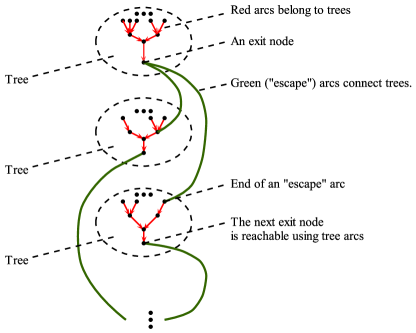
\includegraphics[width=0.85\linewidth,height=0.5\textheight,keepaspectratio]{x2.png}\end{center}
 
Figure 1: Structure of a connected cofinal subgraph of a connected component of a confluent ARS of the least uncountable cardinality, assuming this component lacks the cofinality property.\par
 
% END S5.F1
 
% BEGIN S5.F2

\begin{center}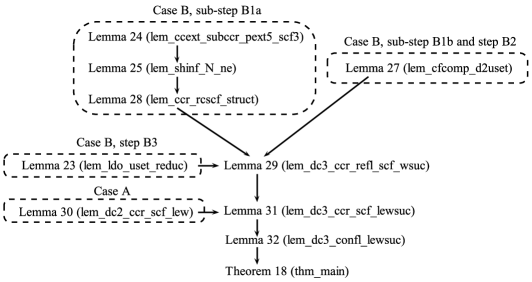
\includegraphics[width=0.85\linewidth,height=0.5\textheight,keepaspectratio]{x3.png}\end{center}
 
Figure 2: An approximate correspondence between the cases/steps from subsection 5.1 and lemmas used in the proof of the main result. Arrows $A\to B$ mean that $A$ is used in the proof of $B$. Lemmas are denoted as follows: “Name of a lemma in the paper (name of a formal version in [17])”.\par
 
% END S5.F2
 
% END S5.SS1
 
% BEGIN S5.SS2
 
\par\medskip\noindent\textbf{5.2 Formalization of finite levels of the DCR hierarchy}\par
 
% BEGIN S5.SS2.p1
 
In this subsection we describe the way in which finite levels of the DCR hierarchy, i.e. classes $DCR_{\alpha}$ for ordinals $\alpha<\omega$, are formalized in [17].\par
 
% END S5.SS2.p1
 
% BEGIN S5.SS2.p2
 
For any relation $s\subseteq U\times U$ we will denote as $s^{=}$ and $s^{*}$ the reflexive, and, respectively, reflexive transitive closure of $s$ on the set $U$.\par
 
% END S5.SS2.p2
 
% BEGIN S5.SS2.p3
 
For any function $g:[0,\omega)\to 2^{U\times U}$ and any ordinals $\alpha,\beta\in[0,\omega)$ let us denote:\par
  
\par\noindent  $\blacksquare$ 
% BEGIN S5.I3.i1.p1
 
$\mathfrak{L}_{1}(g,\alpha)=\bigcup_{\alpha^{\prime}\in[0,\alpha)}g(\alpha^{%
\prime})$\par
 
% END S5.I3.i1.p1
 
 
\par\noindent  $\blacksquare$ 
% BEGIN S5.I3.i2.p1
 
$\mathfrak{L}_{\vee}(g,\alpha,\beta)=\bigcup_{\alpha^{\prime}\in[0,\alpha)\cup[%
0,\beta)}g(\alpha^{\prime})$\par
 
% END S5.I3.i2.p1
 
 
\par\noindent  $\blacksquare$ 
% BEGIN S5.I3.i3.p1
 
$\mathfrak{D}(g,\alpha,\beta)$ is the set of all tuples $(b,b^{\prime},b^{\prime\prime},d)\in U\times U\times U\times U$ such that\par
    \[(b,b^{\prime})\in(\mathfrak{L}_{1}(g,\alpha))^{*}\leavevmode\nobreak\ \wedge%
\leavevmode\nobreak\ (b^{\prime},b^{\prime\prime})\in(g(\beta))^{=}\leavevmode%
\nobreak\ \wedge\leavevmode\nobreak\ (b^{\prime\prime},d)\in(\mathfrak{L}_{%
\vee}(g,\alpha,\beta))^{*}.\]    
% END S5.I3.i3.p1
 
  
% END S5.SS2.p3
 
% BEGIN Thmtheorem20
 
\par\medskip\noindent\textbf{Definition 20.}\par
 
% BEGIN Thmtheorem20.p1
 
A function $g:[0,\omega)\to 2^{U\times U}$ is called DCR-generating, if for every $\alpha,\beta\in[0,\omega)$ and every $a,b,c\in U$ the following implication holds: if $(a,b)\in g(\alpha)\wedge(a,c)\in g(\beta)$, then there exist $b^{\prime},b^{\prime\prime},c^{\prime},c^{\prime\prime},d\in U$ such that\par
    \[(b,b^{\prime},b^{\prime\prime},d)\in\mathfrak{D}(g,\alpha,\beta)\wedge(c,c^{%
\prime},c^{\prime\prime},d)\in\mathfrak{D}(g,\beta,\alpha).\]    
% END Thmtheorem20.p1
 
% END Thmtheorem20
 
% BEGIN S5.SS2.p4
 
Let us denote:\par
  
\par\noindent  $\blacksquare$ 
% BEGIN S5.I4.i1.p1
 
$DCR_{n}(U)$, where $n\in[0,\omega)$, is the set of all relations $r\subseteq U\times U$ such that there exists a DCR-generating function $g$ such that $r=\bigcup_{\alpha\in[0,n)}g(\alpha)$.\par
 
% END S5.I4.i1.p1
 
  
% END S5.SS2.p4
 
% BEGIN Thmtheorem21
 
\par\medskip\noindent\textbf{$\blacktriangleright$ Remark 21.}\par
 
% BEGIN Thmtheorem21.p1
 
It is straightforward to check that for every $n\in[0,\omega)$, a relation $r$ belongs to $DCR_{n}(U)$ if and only if the ARS $(U,r)$ belongs to the class $DCR_{n}$.\par
 
% END Thmtheorem21.p1
 
% END Thmtheorem21
 
% BEGIN Thmtheorem22
 
\par\medskip\noindent\textbf{Definition 22.}\par
 
% BEGIN Thmtheorem22.p1
 
A binary relation $r\subseteq U\times U$ is called\par
  
\par\noindent  1. 
% BEGIN S5.I5.i1.p1
 
connected Church-Rosser (CCR), if $\forall a,b\in\mathrm{Fld}(r)\leavevmode\nobreak\ \exists c\in\mathrm{Fld}(r)%
\leavevmode\nobreak\ (a,c)\in r^{*}\wedge(b,c)\in r^{*}$\par
 
% END S5.I5.i1.p1
 
 
\par\noindent  2. 
% BEGIN S5.I5.i2.p1
 
cone-like, if $r=\emptyset\vee(\exists m\in\mathrm{Fld}(r)\leavevmode\nobreak\ \forall a\in%
\mathrm{Fld}(r)\leavevmode\nobreak\ (a,m)\in r^{*})$.\par
 
% END S5.I5.i2.p1
 
  
% END Thmtheorem22.p1
 
% END Thmtheorem22
 
% BEGIN S5.SS2.p5
 
We will denote:\par
  
\par\noindent  $\blacksquare$ 
% BEGIN S5.I6.i1.p1
 
$CCR(U)$ is the set of all CCR relations $r\subseteq U\times U$\par
 
% END S5.I6.i1.p1
 
 
\par\noindent  $\blacksquare$ 
% BEGIN S5.I6.i2.p1
 
$Conelike(U)$ is the set of all cone-like relations $r\subseteq U\times U$.\par
 
% END S5.I6.i2.p1
 
  
% END S5.SS2.p5
 
% BEGIN S5.SS2.p6
 
For any $r\subseteq U\times U$ let us denote:\par
  
\par\noindent  $\blacksquare$ 
% BEGIN S5.I7.i1.p1
 
$\mathfrak{U}(r)=\{s\in CCR(U)\leavevmode\nobreak\ |\leavevmode\nobreak\ s%
\subseteq r\leavevmode\nobreak\ \wedge\leavevmode\nobreak\ \forall a\in\mathrm%
{Fld}(r)\leavevmode\nobreak\ \exists b\in\mathrm{Fld}(s)\leavevmode\nobreak\ (%
a,b)\in r^{*}\}$. We will call any element of $\mathfrak{U}(r)$ a CCR residue of $r$.\par
 
% END S5.I7.i1.p1
 
  
% END S5.SS2.p6
 
% BEGIN S5.SS2.p7
 
Note that a CCR residue of $r$ is a CCR subrelation $s\subseteq r$ such that the field of $s$ is a cofinal subset in the preordered set $(\mathrm{Fld}(r),r^{*}|_{\mathrm{Fld}(r)})$.\par
 
% END S5.SS2.p7
 
% BEGIN S5.SS2.p8
 
The next lemma will be used to implement the step “B3” from subsection 5.1 (it can be considered as a restricted version of a theorem about DCR hierarchy presented in [20]).\par
 
% END S5.SS2.p8
 
% BEGIN Thmtheorem23
 
\par\medskip\noindent\textbf{Lemma 23 (DCR property inference using CCR residue argument).}\par
 
% BEGIN Thmtheorem23.p1
 
If $n_{0}\in[1,\omega)$, $r\subseteq U\times U$, $s\in\mathfrak{U}(r)$, and $s\in DCR_{n_{0}}(U)$, then $r\in DCR_{n_{0}+1}(U)$.\par
 
% END Thmtheorem23.p1
 
% END Thmtheorem23
 
% BEGIN S5.SS2.SSS0.P0.SPx1
 
\par\medskip\noindent\textbf{Proof.}\par
 
% BEGIN S5.SS2.SSS0.P0.SPx1.p1
 
A formal proof is available in [17, lines 7275–7598]. The proof involves extraction of an auxiliary spanning subrelation of $r$ entitled r1 [17, line 7458, 7590], labeling r1 to show that $\texttt{r1}\in DCR_{n_{0}}(U)$ as described in [17, lines 7450–7453, 7588, 7591], and extension of a labeling of r1 to a labeling of $r$ that ensures that $r\in DCR_{n_{0}+1}(U)$ [17, line 7597]. $\hfill\blacktriangleleft$\par
 
% END S5.SS2.SSS0.P0.SPx1.p1
 
% END S5.SS2.SSS0.P0.SPx1
 
% END S5.SS2
 
% BEGIN S5.SS3
 
\par\medskip\noindent\textbf{5.3 CCR relation subfield extension lemma}\par
 
% BEGIN S5.SS3.p1
 
For any $r\subseteq U\times U$, $A\subseteq U$, and $x\in U$ let us denote:\par
  
\par\noindent  $\blacksquare$ 
% BEGIN S5.I8.i1.p1
 
$r\left[A\right]=\{b\leavevmode\nobreak\ |\leavevmode\nobreak\ \exists a\in A%
\leavevmode\nobreak\ (a,b)\in r\}$, i.e. $r\left[A\right]$ is the image of $A$ under $r$\par
 
% END S5.I8.i1.p1
 
 
\par\noindent  $\blacksquare$ 
% BEGIN S5.I8.i2.p1
 
$r\{x\}=\{y\leavevmode\nobreak\ |\leavevmode\nobreak\ (x,y)\in r\}$, i.e. $r\{x\}$ is the set of successors of $x$ w.r.t. $r$\par
 
% END S5.I8.i2.p1
 
 
\par\noindent  $\blacksquare$ 
% BEGIN S5.I8.i3.p1
 
$\mathrm{dncl}(r,A)=((r^{*})^{-1})[A]$, i.e. $\mathrm{dncl}(r,A)$ is the downward closure of $A$ in $(U,r^{*})$\par
 
% END S5.I8.i3.p1
 
 
\par\noindent  $\blacksquare$ 
% BEGIN S5.I8.i4.p1
 
$Inv(r)=\{A\subseteq U\leavevmode\nobreak\ |\leavevmode\nobreak\ r\left[A\right%
]\subseteq A\leavevmode\nobreak\ \}$, elements of $Inv(r)$ are called invariant sets of $r$\par
 
% END S5.I8.i4.p1
 
 
\par\noindent  $\blacksquare$ 
% BEGIN S5.I8.i5.p1
 
$Span(r)=\{s\subseteq r\leavevmode\nobreak\ |\leavevmode\nobreak\ \mathrm{Fld}(%
s)=\mathrm{Fld}(r)\}$, elements of $Span(r)$ are called spanning subrelations of $r$\par
 
% END S5.I8.i5.p1
 
 
\par\noindent  $\blacksquare$ 
% BEGIN S5.I8.i6.p1
 
$SF(r)=\{A\subseteq U\leavevmode\nobreak\ |\leavevmode\nobreak\ \mathrm{Fld}(r|%
_{A})=A\leavevmode\nobreak\ \}$, elements of $SF(r)$ are called subfields of $r$ (note that $A$ is a subfield of $r$ if and only if $A$ is the field of some subrelation $s\subseteq r$)\par
 
% END S5.I8.i6.p1
 
 
\par\noindent  $\blacksquare$ 
% BEGIN S5.I8.i7.p1
 
$SCF(r)=\{\,B\subseteq\mathrm{Fld}(r)\leavevmode\nobreak\ |\leavevmode\nobreak%
\ \forall a\in\mathrm{Fld}(r)\leavevmode\nobreak\ \exists b\in B\leavevmode%
\nobreak\ (a,b)\in r^{*}\}$, i.e. $SCF(r)$ is the set of all cofinal sets in the preordered set $(\mathrm{Fld}(r),r^{*}|_{\mathrm{Fld}(r)})$\par
 
% END S5.I8.i7.p1
 
 
\par\noindent  $\blacksquare$ 
% BEGIN S5.I8.i8.p1
 
$\mathrm{scf}(r)=\min\{\leavevmode\nobreak\ |B|\leavevmode\nobreak\ |%
\leavevmode\nobreak\ B\in SCF(r)\leavevmode\nobreak\ \}$, here $\mathrm{scf}(r)$ is called the sequential cofinality of $r$.\par
 
% END S5.I8.i8.p1
 
  
% END S5.SS3.p1
 
% BEGIN S5.SS3.p2
 
For any set $X$ denote as $\mathcal{P}(X)$ the set of all subsets of $X$.\par
 
% END S5.SS3.p2
 
% BEGIN S5.SS3.p3
 
Let us fix a (choice) function $\mathrm{ch}:\mathcal{P}(\mathcal{P}(U))\backslash\{\emptyset\}\to\mathcal{P}(U)$ such that $\mathrm{ch}(A)\in A$ for every nonempty set $A\subseteq\mathcal{P}(U)$.\par
 
% END S5.SS3.p3
 
% BEGIN S5.SS3.p4
 
For any $r,s^{\prime}\subseteq U\times U$, $A,B\subseteq U$, and $a,b\in U$ let us denote:\par
  
\par\noindent  $\blacksquare$ 
% BEGIN S5.I9.i1.p1
 
$\mathcal{F}(r,a,b)$ is the set of all (finite) subsets $F\subseteq U$ such that there exists a non-negative integer $n$ and a finite sequence $(a_{i})_{i=0}^{n}$ of elements of $U$ such that $F=\{a_{0},a_{1},...,a_{n}\}$, $a_{0}=a$, $a_{n}=b$, and $(a_{i},a_{i+1})\in r$ for all $i=0,1,...,n-1$\par
 
% END S5.I9.i1.p1
 
 
\par\noindent  $\blacksquare$ 
% BEGIN S5.I9.i2.p1
 
$\mathrm{wdncl}(r,A)=\{a\in\mathrm{dncl}(r,A)\leavevmode\nobreak\ |\leavevmode%
\nobreak\ \forall b\in U\leavevmode\nobreak\ \forall F\in\mathcal{F}(r,a,b)%
\leavevmode\nobreak\ (b\notin\mathrm{dncl}(r,A)\Rightarrow F\cap A\neq%
\emptyset)\}$\par
 
% END S5.I9.i2.p1
 
 
\par\noindent  $\blacksquare$ 
% BEGIN S5.I9.i3.p1
 
$\mathrm{wrank}(r,A)=\min\{\leavevmode\nobreak\ |B|\leavevmode\nobreak\ |%
\leavevmode\nobreak\ A\subseteq\mathrm{wdncl}(r,B)\leavevmode\nobreak\ \}$\par
 
% END S5.I9.i3.p1
 
 
\par\noindent  $\blacksquare$ 
% BEGIN S5.I9.i4.p1
 
$\mathrm{dn_{Esc}}(r,A,a)=\{\leavevmode\nobreak\ F\in\mathcal{P}(U)\leavevmode%
\nobreak\ |\leavevmode\nobreak\ \exists b\in U\backslash\mathrm{dncl}(r,A)%
\leavevmode\nobreak\ F\in\mathcal{F}(r,a,b)\wedge(F\cap A=\emptyset)%
\leavevmode\nobreak\ \}$\par
 
% END S5.I9.i4.p1
 
 
\par\noindent  $\blacksquare$ 
% BEGIN S5.I9.i5.p1
 
$\mathrm{dn_{esc}}(r,A,a)=\begin{cases}\mathrm{ch}(\mathrm{dn_{Esc}}(r,A,a)),&%
\text{ if }\mathrm{dn_{Esc}}(r,A,a)\neq\emptyset\\
\{a\},&\text{ if }\mathrm{dn_{Esc}}(r,A,a)=\emptyset\\
\end{cases}$\par
 
% END S5.I9.i5.p1
 
 
\par\noindent  $\blacksquare$ 
% BEGIN S5.I9.i6.p1
 
$\mathrm{escl}(r,A,B)=\bigcup_{b\in B}\mathrm{dn_{esc}}(r,A,b)$\par
 
% END S5.I9.i6.p1
 
 
\par\noindent  $\blacksquare$ 
% BEGIN S5.I9.i7.p1
 
$\mathrm{clterm}(s^{\prime},r)=(s^{\prime}\in Conelike(U)\Rightarrow r\in
Conelike%
(U))$.\par
 
% END S5.I9.i7.p1
 
  
% END S5.SS3.p4
 
% BEGIN Thmtheorem24
 
\par\medskip\noindent\textbf{Lemma 24.}\par
 
% BEGIN Thmtheorem24.p1
 
Let $r\in CCR(U)$, $A\in SF(r)$, $B,B^{\prime}\subseteq U$, $x\in U$, and $Ps\subseteq SCF(r)$.\par
 
% END Thmtheorem24.p1
 
% BEGIN Thmtheorem24.p2
 
Then there exists a set $A^{\prime}\subseteq U$ that satisfies of the following 9 conditions:\par
  
\par\noindent  1. 
% BEGIN S5.I10.i1.p1
 
$x\in\mathrm{Fld}(r)\Rightarrow x\in A^{\prime}$\par
 
% END S5.I10.i1.p1
 
 
\par\noindent  2. 
% BEGIN S5.I10.i2.p1
 
$A\subseteq A^{\prime}$\par
 
% END S5.I10.i2.p1
 
 
\par\noindent  3. 
% BEGIN S5.I10.i3.p1
 
$A^{\prime}\in SF(r)$\par
 
% END S5.I10.i3.p1
 
 
\par\noindent  4. 
% BEGIN S5.I10.i4.p1
 
$\forall a\in A\leavevmode\nobreak\ ((r\{a\}\subseteq B)\leavevmode\nobreak\ %
\vee\leavevmode\nobreak\ (r\{a\}\cap(A^{\prime}\backslash B)\neq\emptyset))$\par
 
% END S5.I10.i4.p1
 
 
\par\noindent  5. 
% BEGIN S5.I10.i5.p1
 
$(\exists y\in U\leavevmode\nobreak\ A^{\prime}-B^{\prime}\subseteq\{y\})%
\Rightarrow(\mathrm{Fld}(r)\subseteq A^{\prime}\cup B^{\prime})$\par
 
% END S5.I10.i5.p1
 
 
\par\noindent  6. 
% BEGIN S5.I10.i6.p1
 
$r|_{A^{\prime}}\in CCR(U)$\par
 
% END S5.I10.i6.p1
 
 
\par\noindent  7. 
% BEGIN S5.I10.i7.p1
 
$(|A|<\omega\Rightarrow|A^{\prime}|<\omega)\wedge(|A|\geq\omega\Rightarrow|A^{%
\prime}|=|A|)$\par
 
% END S5.I10.i7.p1
 
 
\par\noindent  8. 
% BEGIN S5.I10.i8.p1
 
$((\exists P\leavevmode\nobreak\ Ps=\{P\})\,\vee\leavevmode\nobreak\ |Ps|\in[%
\omega,|A|\,])\Rightarrow(\forall P\in Ps\leavevmode\nobreak\ (A^{\prime}\cap P%
)\in SCF(r|_{A^{\prime}}))$\par
 
% END S5.I10.i8.p1
 
 
\par\noindent  9. 
% BEGIN S5.I10.i9.p1
 
$|A|\geq\omega\Rightarrow\mathrm{escl}(r,A,A^{\prime})\subseteq A^{\prime}%
\wedge\mathrm{clterm}(r|_{A^{\prime}},r)$.\par
 
% END S5.I10.i9.p1
 
  
% END Thmtheorem24.p2
 
% END Thmtheorem24
 
% BEGIN S5.SS3.SSS0.P0.SPx1
 
\par\medskip\noindent\textbf{Proof.}\par
 
% BEGIN S5.SS3.SSS0.P0.SPx1.p1
 
A formal proof is available in [17, lines 4498–4538]. It depends on several auxiliary formal lemmas that have close formulations, but provide weaker/different guarantees (lem\_Ccext\_finsubccr\_pext5\_scf3 and lem\_Ccext\_infsubccr\_pext5\_scf3 in [17] and their dependencies). The idea of the proof of the current lemma and its dependencies is related to Löwenheim-Skolem theorem.\par
 
% END S5.SS3.SSS0.P0.SPx1.p1
 
% BEGIN S5.SS3.SSS0.P0.SPx1.p2
 
When $A$ is infinite, the proof aims to define a required set $A^{\prime}$ as\par
    \[\psi\left(\bigcup_{n=0}^{\infty}H^{(n)}(\phi(A))\right),\]  (2)   
for some suitable increasing set function $H$ and set functions $\phi$, $\psi$, where $H^{(n)}$ denotes the $n$-times composition of $H$ with itself, such that $H$, $\phi$, $\psi$ ensure closure properties of $A^{\prime}$ required by the lemma’s conditions (e.g. $r|_{A^{\prime}}\in CCR(U)$), but keep the cardinalities of sets defined by subexpressions of (2) bounded, so that the condition 7, i.e. $(|A|<\omega\Rightarrow|A^{\prime}|<\omega)\wedge(|A|\geq\omega\Rightarrow|A^{%
\prime}|=|A|)$, holds. An explicit expression for $\phi(A)$ can be obtained by unfolding the notation on the right hand side of the definition in [17, line 3972], taking into account substitutions of values in place of parameters of the auxiliary lemma lem\_Ccext\_infsubccr\_set\_ext\_scf3 specified in [17, line 4280]. Similarly, $H$ can be expressed by unfolding the notation used in [17, lines 3964–3966], and as $\psi$ one can take the identity function.\par
 
% END S5.SS3.SSS0.P0.SPx1.p2
 
% BEGIN S5.SS3.SSS0.P0.SPx1.p3
 
If $A$ is a finite set, the proof is based on induction on the size of an auxiliary finite relation associated with $A$. Details can be found in [17, lines 4372–4496, 3332–3414, 2485–2680]. $\hfill\blacktriangleleft$\par
 
% END S5.SS3.SSS0.P0.SPx1.p3
 
% END S5.SS3.SSS0.P0.SPx1
 
% END S5.SS3
 
% BEGIN S5.SS4
 
\par\medskip\noindent\textbf{5.4 Analog of Iwamura’s lemma on directed sets for CCR relations}\par
 
% BEGIN S5.SS4.p1
 
In this subsection we describe a lemma that allows one to represent an infinite CCR relation $r$ as a union of a chain of CCR relations of cardinalities smaller than the cardinality of $r$ in a way reminiscent to Iwamura’s lemma on directed sets [29, Theorem 1]. Unlike Iwamura’s lemma, our lemma is applicable to a not-necessarily-transitive CCR relation $r$ and guarantees that fields of elements of the resulting chain satisfy additional constraints described below using the sets $\mathcal{N}_{i}$ that are used in the proof of the main result.\par
 
% END S5.SS4.p1
 
% BEGIN S5.SS4.p2
 
Let $\mathcal{U}$ be the set of all ordinals of the cardinality at most $|U|$.\par
 
% END S5.SS4.p2
 
% BEGIN S5.SS4.p3
 
For any $f:\mathcal{U}\to 2^{U}$ and ordinal $\alpha\in\mathcal{U}$ let us denote:\par
  
\par\noindent  $\blacksquare$ 
% BEGIN S5.I11.i1.p1
 
$\mathfrak{L}(f,\alpha)=\bigcup_{\alpha^{\prime}\in[0,\alpha)}f(\alpha^{\prime})$\par
 
% END S5.I11.i1.p1
 
 
\par\noindent  $\blacksquare$ 
% BEGIN S5.I11.i2.p1
 
$\nabla(f,\alpha)=f(\alpha)\backslash\mathfrak{L}(f,\alpha)$\par
 
% END S5.I11.i2.p1
 
 
\par\noindent  $\blacksquare$ 
% BEGIN S5.I11.i3.p1
 
$\mathcal{Q}(r,f,\alpha)=f(\alpha)\backslash\mathrm{dncl}(r,\mathfrak{L}(f,%
\alpha))$\par
 
% END S5.I11.i3.p1
 
 
\par\noindent  $\blacksquare$ 
% BEGIN S5.I11.i4.p1
 
$\mathcal{W}(r,f,\alpha)=f(\alpha)\backslash\mathrm{wdncl}(r,\mathfrak{L}(f,%
\alpha))$.\par
 
% END S5.I11.i4.p1
 
  
% END S5.SS4.p3
 
% BEGIN S5.SS4.p4
 
For any $r\subseteq U\times U$, $Ps\subseteq 2^{U}$, and ordinal $\alpha_{0}\in\mathcal{U}$ let us denote:\par
  
\par\noindent  $\blacksquare$ 
% BEGIN S5.I12.i1.p1
 
$\mathcal{N}_{1}(r,\alpha_{0})=\{\leavevmode\nobreak\ f:\mathcal{U}\to 2^{U}%
\leavevmode\nobreak\ |\leavevmode\nobreak\ \forall\alpha\in[0,\alpha_{0}]%
\leavevmode\nobreak\ \forall\alpha^{\prime}\in[0,\alpha]\leavevmode\nobreak\ f%
(\alpha^{\prime})\subseteq f(\alpha)\leavevmode\nobreak\ \}$\par
 
% END S5.I12.i1.p1
 
 
\par\noindent  $\blacksquare$ 
% BEGIN S5.I12.i2.p1
 
$\mathcal{N}_{2}(r,\alpha_{0})=\{\leavevmode\nobreak\ f:\mathcal{U}\to 2^{U}%
\leavevmode\nobreak\ |\leavevmode\nobreak\ \forall\alpha\in[0,\alpha_{0}]_{L}%
\leavevmode\nobreak\ \nabla(f,\alpha)=\emptyset\leavevmode\nobreak\ \}$\par
 
% END S5.I12.i2.p1
 
 
\par\noindent  $\blacksquare$ 
% BEGIN S5.I12.i3.p1
 
$\mathcal{N}_{3}(r,\alpha_{0})=\{\leavevmode\nobreak\ f:\mathcal{U}\to 2^{U}%
\leavevmode\nobreak\ |\leavevmode\nobreak\ \forall\alpha\in[0,\alpha_{0}]_{0S}%
\leavevmode\nobreak\ \leavevmode\nobreak\ |\mathfrak{L}(f,\alpha)|\geq\omega\Rightarrow$\par
 
% END S5.I12.i3.p1
 
% BEGIN S5.I12.i3.p2
 
$\leavevmode\nobreak\ (\leavevmode\nobreak\ \mathrm{escl}(r,\mathfrak{L}(f,%
\alpha),f(\alpha))\subseteq f(\alpha)\leavevmode\nobreak\ \wedge\leavevmode%
\nobreak\ \mathrm{clterm}(r|_{f(\alpha)},r)\leavevmode\nobreak\ )\leavevmode%
\nobreak\ \}$\par
 
% END S5.I12.i3.p2
 
 
\par\noindent  $\blacksquare$ 
% BEGIN S5.I12.i4.p1
 
$\mathcal{N}_{4}(r,\alpha_{0})=\{\leavevmode\nobreak\ f:\mathcal{U}\to 2^{U}%
\leavevmode\nobreak\ |\leavevmode\nobreak\ \forall\alpha\in[0,\alpha_{0}]_{0S}%
\leavevmode\nobreak\ $  $\forall a\in\mathfrak{L}(f,\alpha)\leavevmode\nobreak\ (\leavevmode\nobreak\ r%
\{a\}\subseteq\mathrm{wdncl}(r,\mathfrak{L}(f,\alpha))\leavevmode\nobreak\ %
\vee\leavevmode\nobreak\ (r\{a\}\cap\mathcal{W}(r,f,\alpha)\neq\emptyset)%
\leavevmode\nobreak\ )\leavevmode\nobreak\ \}$\par
 
% END S5.I12.i4.p1
 
 
\par\noindent  $\blacksquare$ 
% BEGIN S5.I12.i5.p1
 
$\mathcal{N}_{5}(r,\alpha_{0})=\{\leavevmode\nobreak\ f:\mathcal{U}\to 2^{U}%
\leavevmode\nobreak\ |\leavevmode\nobreak\ \forall\alpha\in[0,\alpha_{0}]%
\leavevmode\nobreak\ f(\alpha)\in SF(r)\,\leavevmode\nobreak\ \}$\par
 
% END S5.I12.i5.p1
 
 
\par\noindent  $\blacksquare$ 
% BEGIN S5.I12.i6.p1
 
$\mathcal{N}_{6}(r,\alpha_{0})=\{\leavevmode\nobreak\ f:\mathcal{U}\to 2^{U}%
\leavevmode\nobreak\ |\leavevmode\nobreak\ \forall\alpha\in[0,\alpha_{0}]%
\leavevmode\nobreak\ r|_{f(\alpha)}\in CCR(U)\leavevmode\nobreak\ \}$\par
 
% END S5.I12.i6.p1
 
 
\par\noindent  $\blacksquare$ 
% BEGIN S5.I12.i7.p1
 
$\mathcal{N}_{7}(r,\alpha_{0})=\{\leavevmode\nobreak\ f:\mathcal{U}\to 2^{U}%
\leavevmode\nobreak\ |\leavevmode\nobreak\ \forall\alpha\in[0,\alpha_{0}]%
\leavevmode\nobreak\ $  $(\leavevmode\nobreak\ (\alpha<\omega\Rightarrow|f(\alpha)|<\omega)\wedge(%
\alpha\geq\omega\Rightarrow|f(\alpha)|\leq\alpha)\leavevmode\nobreak\ )%
\leavevmode\nobreak\ \}$\par
 
% END S5.I12.i7.p1
 
 
\par\noindent  $\blacksquare$ 
% BEGIN S5.I12.i8.p1
 
$\mathcal{N}_{8}(r,Ps,\alpha_{0})=\{\leavevmode\nobreak\ f:\mathcal{U}\to 2^{U}%
\leavevmode\nobreak\ |\leavevmode\nobreak\ \forall\alpha\in[0,\alpha_{0}]_{0S}%
\leavevmode\nobreak\ $  $(\leavevmode\nobreak\ (|Ps|=1\leavevmode\nobreak\ \vee\leavevmode\nobreak\ |Ps%
|\in[\omega,|f(\alpha)|\,])\Rightarrow(\forall P\in Ps\leavevmode\nobreak\ (f(%
\alpha)\cap P)\in SCF(r|_{f(\alpha)}))\leavevmode\nobreak\ )\leavevmode%
\nobreak\ \}$\par
 
% END S5.I12.i8.p1
 
 
\par\noindent  $\blacksquare$ 
% BEGIN S5.I12.i9.p1
 
$\mathcal{N}_{9}(r,\alpha_{0})=\{\leavevmode\nobreak\ f:\mathcal{U}\to 2^{U}%
\leavevmode\nobreak\ |\leavevmode\nobreak\ \alpha_{0}\geq\omega\Rightarrow\,%
\mathrm{Fld}(r)\subseteq f(\alpha_{0})\leavevmode\nobreak\ \}$\par
 
% END S5.I12.i9.p1
 
 
\par\noindent  $\blacksquare$ 
% BEGIN S5.I12.i10.p1
 
$\mathcal{N}_{10}(r,\alpha_{0})=\{\leavevmode\nobreak\ f:\mathcal{U}\to 2^{U}%
\leavevmode\nobreak\ |\leavevmode\nobreak\ \forall\alpha\in[0,\alpha_{0}]$  $((\,\exists y\in U\leavevmode\nobreak\ \mathcal{Q}(r,f,\alpha)=\{y\}\,)%
\Rightarrow\,\mathrm{Fld}(r)\subseteq\mathrm{dncl}(r,f(\alpha))\,)\leavevmode%
\nobreak\ \}$\par
 
% END S5.I12.i10.p1
 
 
\par\noindent  $\blacksquare$ 
% BEGIN S5.I12.i11.p1
 
$\mathcal{N}_{11}(r,\alpha_{0})=\{\leavevmode\nobreak\ f:\mathcal{U}\to 2^{U}%
\leavevmode\nobreak\ |\leavevmode\nobreak\ \forall\alpha\in[0,\alpha_{0}]_{0S}%
\backslash\{0\}$  $(\mathcal{Q}(r,f,\alpha)=\emptyset\,\Rightarrow\,\mathrm{Fld}(r)\subseteq%
\mathrm{dncl}(r,f(\alpha))\,)\leavevmode\nobreak\ \}$\par
 
% END S5.I12.i11.p1
 
 
\par\noindent  $\blacksquare$ 
% BEGIN S5.I12.i12.p1
 
$\mathcal{N}_{12}(r,\alpha_{0})=\{\leavevmode\nobreak\ f:\mathcal{U}\to 2^{U}%
\leavevmode\nobreak\ |\leavevmode\nobreak\ \forall\alpha\in[\omega,\alpha_{0}]%
\leavevmode\nobreak\ |\mathfrak{L}(f,\alpha)|\geq\omega\leavevmode\nobreak\ \}$.\par
 
% END S5.I12.i12.p1
 
  
% END S5.SS4.p4
 
% BEGIN S5.SS4.p5
 
For every $r\subseteq U\times U$ and $Ps\subseteq 2^{U}$ let us denote:\par
    \[\mathcal{N}(r,Ps)=\left(\bigcap_{i=1}^{7}\mathcal{N}_{i}(r,|\mathrm{Fld}(r)|)%
\right)\cap\mathcal{N}_{8}(r,Ps,|\mathrm{Fld}(r)|)\cap\left(\bigcap_{i=9}^{12}%
\mathcal{N}_{i}(r,|\mathrm{Fld}(r)|)\right).\]  (3)   
Note that $|\mathrm{Fld}(r)|\in[0,|U|\,]\subseteq\mathcal{U}$, because $\mathrm{Fld}(r)\subseteq U$.\par
 
% END S5.SS4.p5
 
% BEGIN Thmtheorem25
 
\par\medskip\noindent\textbf{Lemma 25 (Analog of Iwamura’s lemma).}\par
 
% BEGIN Thmtheorem25.p1
 
If $r\in CCR(U)$ and $Ps\subseteq SCF(r)$, then $\mathcal{N}(r,Ps)\neq\emptyset$.\par
 
% END Thmtheorem25.p1
 
% END Thmtheorem25
 
% BEGIN S5.SS4.SSS0.P0.SPx1
 
\par\medskip\noindent\textbf{Proof.}\par
 
% BEGIN S5.SS4.SSS0.P0.SPx1.p1
 
A formal proof is available in [17, lines 9533–9616]. The idea of the proof is to use Lemma 24 to define recursively a transfinite sequence of subsets of $\mathrm{Fld}(r)$ that gives values $f(\alpha)$, $\alpha\in[0,|\mathrm{Fld}(r)|]$ for some $f\in\mathcal{N}(r,Ps)$. $\hfill\blacktriangleleft$\par
 
% END S5.SS4.SSS0.P0.SPx1.p1
 
% BEGIN Thmtheorem26
 
\par\medskip\noindent\textbf{$\blacktriangleright$ Remark 26.}\par
 
% BEGIN Thmtheorem26.p1
 
If $f\in\mathcal{N}(r,Ps)$ for an infinite CCR relation $r$, then the relations $r|_{f(\alpha)}$, $\alpha\in[0,|\mathrm{Fld}(r)|)$ are smaller than $r$ in cardinality and form a chain of CCR relations, the union of which is $r$ (one can check this by unfolding the notations $\mathcal{N}_{i}(r,|\mathrm{Fld}(r)|)$ for $i=1,2,5,6,7,9$ and $\nabla(f,\alpha)$ and noting that if $r$ is infinite, then $|\mathrm{Fld}(r)|$ is a limit ordinal).\par
 
% END Thmtheorem26.p1
 
% END Thmtheorem26
 
% END S5.SS4.SSS0.P0.SPx1
 
% END S5.SS4
 
% BEGIN S5.SS5
 
\par\medskip\noindent\textbf{5.5 Generation of a CCR residue in the class DCR2}\par
 
% BEGIN S5.SS5.p1
 
Let us denote:\par
  
\par\noindent  $\blacksquare$ 
% BEGIN S5.I13.i1.p1
 
$T(U)$ is the set of all nonempty relations $t\in CCR(U)$ such that $t$ is single-valued (i.e. $(a,b)\in t\wedge(a,c)\in t\Rightarrow b=c$), acyclic (i.e. $t^{+}$ is irreflexive), and total on its field (i.e. $\forall x\in\mathrm{Fld}(t)\leavevmode\nobreak\ t\{x\}\neq\emptyset$).\par
 
% END S5.I13.i1.p1
 
  
% END S5.SS5.p1
 
% BEGIN Thmtheorem27
 
\par\medskip\noindent\textbf{Lemma 27.}\par
 
% BEGIN Thmtheorem27.p1
 
Let $r\subseteq U\times U$ be a relation that is reflexive on $\mathrm{Fld}(r)$. Let $S$ be a set of ordinals and $(W_{\alpha})_{\alpha\in S}$, $(R_{\alpha})_{\alpha\in S}$ be indexed families of subsets of $U$ such that\par
  
\par\noindent  1. 
% BEGIN S5.I14.i1.p1
 
$S\subseteq[0,\omega_{1})$, $|[0,\omega_{1})|\leq|S|$, and $\forall\alpha\in S\leavevmode\nobreak\ \exists\beta\in S\leavevmode\nobreak\ %
\alpha<\beta$\par
 
% END S5.I14.i1.p1
 
 
\par\noindent  2. 
% BEGIN S5.I14.i2.p1
 
$\mathrm{Fld}(r)=\bigcup_{\alpha\in S}W_{\alpha}$ and $\forall\alpha,\beta\in S\leavevmode\nobreak\ (\alpha\neq\beta\Rightarrow W_{%
\alpha}\cap W_{\beta}=\emptyset)$\par
 
% END S5.I14.i2.p1
 
 
\par\noindent  3. 
% BEGIN S5.I14.i3.p1
 
$\forall\alpha\in S\leavevmode\nobreak\ R_{\alpha}\in T(U)\wedge R_{\alpha}%
\subseteq r\wedge|W_{\alpha}|\leq\omega\wedge\mathrm{Fld}(R_{\alpha})=W_{%
\alpha}\wedge\neg Conelike(r|_{W_{\alpha}})$\par
 
% END S5.I14.i3.p1
 
 
\par\noindent  4. 
% BEGIN S5.I14.i4.p1
 
$\forall\alpha\in S\leavevmode\nobreak\ \forall x\in W_{\alpha}\leavevmode%
\nobreak\ \exists a\in U\,\left(\leavevmode\nobreak\ (x,a)\in(r|_{W_{\alpha}})%
^{*}\wedge(\forall\beta\in S\leavevmode\nobreak\ \alpha<\beta\Rightarrow r\{a%
\}\cap W_{\beta}\neq\emptyset)\leavevmode\nobreak\ \right)$.\par
 
% END S5.I14.i4.p1
 
  
% END Thmtheorem27.p1
 
% BEGIN Thmtheorem27.p2
 
Then there exists $r^{\prime}\in\mathfrak{U}(r)$ such that $r^{\prime}\in DCR_{2}(U)$.\par
 
% END Thmtheorem27.p2
 
% END Thmtheorem27
 
% BEGIN S5.SS5.SSS0.P0.SPx1
 
\par\medskip\noindent\textbf{Proof.}\par
 
% BEGIN S5.SS5.SSS0.P0.SPx1.p1
 
A formal proof is available in [17, lines 4935–5746] (note that in the formulation of the lemma in [17] the assumptions are not numbered as above and the notation $\mathfrak{U}(r)$ in the conclusion is unfolded).\par
 
% END S5.SS5.SSS0.P0.SPx1.p1
 
% BEGIN S5.SS5.SSS0.P0.SPx1.p2
 
The idea of the proof is to define a relation $r^{\prime}\in\mathfrak{U}(r)$ (a subrelation of $r$) such that, semi-formally, the graph $(\mathrm{Fld}(r^{\prime}),r^{\prime})$ has a shape similar to the one illustrated in Figure 1, and show that $r^{\prime}\in DCR_{2}(U)$. The trees illustrated in Figure 1 are extracted from (at most countable) graphs $(W_{\alpha},r|_{W_{\alpha}})$ for ordinals $\alpha\in S$.\par
 
% END S5.SS5.SSS0.P0.SPx1.p2
 
% BEGIN S5.SS5.SSS0.P0.SPx1.p3
 
In more detail this construction is described below (the relations $R^{\prime}_{\alpha}$ correspond to sets of arcs of the trees extracted from $(W_{\alpha},r|_{W_{\alpha}})$, the relation $r_{e}^{\prime}$ corresponds to the set of arcs that connect trees, and $r^{\prime}$ is the union of $r^{\prime}_{e}$ and $R^{\prime}_{\alpha}$ for all $\alpha\in S$).\par
 
% END S5.SS5.SSS0.P0.SPx1.p3
 
% BEGIN S5.SS5.SSS0.P0.SPx1.p4
 
For every $\alpha\in S$ let us denote:\par
  
\par\noindent  $\blacksquare$ 
% BEGIN S5.I15.i1.p1
 
$EP_{\alpha}=\{a\in W_{\alpha}\leavevmode\nobreak\ |\leavevmode\nobreak\ %
\forall\beta\in S\leavevmode\nobreak\ (\alpha<\beta\Rightarrow r\{\alpha\}\cap
W%
_{\beta}\neq\emptyset)\}$, the elements of $EP_{\alpha}$ are called exit points from the ARS $(W_{\alpha},r|_{W_{\alpha}})$\par
 
% END S5.I15.i1.p1
 
 
\par\noindent  $\blacksquare$ 
% BEGIN S5.I15.i2.p1
 
$h:\mathcal{U}\to\mathcal{U}$ is a function such that for every $\alpha,\beta\in S$ and $a\in EP_{\alpha}$, $b\in EP_{\beta}$ there exists $\gamma\in S$ and $a^{\prime},b^{\prime}\in W_{\gamma}$ such that $\alpha<\gamma$, $\beta<\gamma$, and $(a,a^{\prime})\in r$, $(a^{\prime},h(\gamma))\in R_{\gamma}^{*}$, $(b,b^{\prime})\in r$, and $(b^{\prime},h(\gamma))\in R_{\gamma}^{*}$\par
 
% END S5.I15.i2.p1
 
 
\par\noindent  $\blacksquare$ 
% BEGIN S5.I15.i3.p1
 
$(s_{\alpha,k})_{k=0}^{\infty}$ is some infinite cofinal reduction sequence in the (countable, CCR) ARS $(\mathrm{Fld}(R_{\alpha}),R_{\alpha})$\par
 
% END S5.I15.i3.p1
 
 
\par\noindent  $\blacksquare$ 
% BEGIN S5.I15.i4.p1
 
$E_{\alpha}=\{(s_{\alpha,k+1},s_{\alpha,k})\notin(r|_{W_{\alpha}})^{*}\}$\par
 
% END S5.I15.i4.p1
 
 
\par\noindent  $\blacksquare$ 
% BEGIN S5.I15.i5.p1
 
$F_{\alpha}=\{s_{\alpha,k}\leavevmode\nobreak\ |\leavevmode\nobreak\ k\in E_{%
\alpha}\}\cap\{a\in W_{\alpha}\leavevmode\nobreak\ |\leavevmode\nobreak\ (h(%
\alpha)\in W_{\alpha}\Rightarrow(h(\alpha),a)\in R_{\alpha}^{*})\wedge(a,h(%
\alpha))\notin R_{\alpha}^{*}\}$\par
 
% END S5.I15.i5.p1
 
 
\par\noindent  $\blacksquare$ 
% BEGIN S5.I15.i6.p1
 
$re_{0,\alpha}$ and $re_{1,\alpha}$ is some pair of consecutive elements in the sequence $(s_{\alpha,k})_{k=0}^{\infty}$ such that $re_{0,\alpha}$ is located at some index $k\in E_{\alpha}$ in $(s_{\alpha,k})_{k=0}^{\infty}$ and $re_{0,\alpha}\in F_{\alpha}$\par
 
% END S5.I15.i6.p1
 
 
\par\noindent  $\blacksquare$ 
% BEGIN S5.I15.i7.p1
 
$ep_{\alpha}$ is some element of $EP_{\alpha}$ such that $(re_{1,\alpha},ep_{\alpha})\in(r|_{W_{\alpha}})^{*}$\par
 
% END S5.I15.i7.p1
 
 
\par\noindent  $\blacksquare$ 
% BEGIN S5.I15.i8.p1
 
${spl}_{\alpha}$ is the length of a shortest reduction sequence in the ARS $(W_{\alpha},r|_{W_{\alpha}})$ that starts at the element ${re}_{1,\alpha}$ and ends at the element ${ep}_{\alpha}$\par
 
% END S5.I15.i8.p1
 
 
\par\noindent  $\blacksquare$ 
% BEGIN S5.I15.i9.p1
 
${sp}_{\alpha,k}$ for $k=0,1,...,({spl}_{\alpha}-1)$ is some reduction sequence that starts at the element ${re}_{1,\alpha}$, ends at the element ${ep}_{\alpha}$, and has the length $spl_{\alpha}$\par
 
% END S5.I15.i9.p1
 
 
\par\noindent  $\blacksquare$ 
% BEGIN S5.I15.i10.p1
 
$R^{\prime}_{\alpha}=\{(a,b)\in R_{\alpha}\leavevmode\nobreak\ |\leavevmode%
\nobreak\ (b,{re}_{0,\alpha})\in R_{\alpha}^{*}\}\cup\{({re}_{0,\alpha},re_{1,%
\alpha})\}\cup\{(sp_{\alpha,k},sp_{\alpha,k+1})\leavevmode\nobreak\ |%
\leavevmode\nobreak\ k<spl_{\alpha}\}$\par
 
% END S5.I15.i10.p1
 
 
\par\noindent  $\blacksquare$ 
% BEGIN S5.I15.i11.p1
 
$r_{e}^{\prime}=\{(a,b)\in r\leavevmode\nobreak\ |\leavevmode\nobreak\ \exists%
\alpha,\beta\in S\leavevmode\nobreak\ \alpha<\beta\wedge a=ep_{\alpha}\wedge b%
\in W_{\beta}\wedge(b,h(\beta))\in R_{\beta}^{*}\}$\par
 
% END S5.I15.i11.p1
 
 
\par\noindent  $\blacksquare$ 
% BEGIN S5.I15.i12.p1
 
$r^{\prime}=r_{e}^{\prime}\cup\bigcup_{\alpha\in S}R^{\prime}_{\alpha}$\par
 
% END S5.I15.i12.p1
 
 
\par\noindent  $\blacksquare$ 
% BEGIN S5.I15.i13.p1
 
$g:[0,\omega)\to 2^{U\times U}$ is a function such that for every $n\in[0,\omega)$:\par
 
% END S5.I15.i13.p1
 
% BEGIN S5.I15.i13.p2
 
$g(n)=\begin{cases}\{(u,v)\in r^{\prime}\leavevmode\nobreak\ |\leavevmode%
\nobreak\ r^{\prime}\{u\}=\{v\}\},&\text{ if }n=0\\
\{(u,v)\in r^{\prime}\leavevmode\nobreak\ |\leavevmode\nobreak\ r^{\prime}\{u%
\}\neq\{v\}\},&\text{ if }n=1\\
\emptyset,&\text{ if }n\notin\{0,1\}.\\
\end{cases}$\par
 
% END S5.I15.i13.p2
 
  
% END S5.SS5.SSS0.P0.SPx1.p4
 
% BEGIN S5.SS5.SSS0.P0.SPx1.p5
 
Then it is shown that $g$ is DCR-generating [17, lines 5659–5720] and $r^{\prime}\in\mathfrak{U}(r)$. Then $r^{\prime}\in\mathfrak{U}(r)\cap DCR_{2}(U)$, because $r^{\prime}=\bigcup_{n<2}g(n)$. $\hfill\blacktriangleleft$\par
 
% END S5.SS5.SSS0.P0.SPx1.p5
 
% END S5.SS5.SSS0.P0.SPx1
 
% END S5.SS5
 
% BEGIN S5.SS6
 
\par\medskip\noindent\textbf{5.6 Completion of the proof of the main theorem}\par
 
% BEGIN S5.SS6.p1
 
Below we give an important lemma (Lemma 28) that can be used to describe a structure of a confluent relation $r$ when $\mathrm{scf}(r)$ is a regular cardinal. We will use it together with several other lemmas to complete the proof of Theorem 18.\par
 
% END S5.SS6.p1
 
% BEGIN Thmtheorem28
 
\par\medskip\noindent\textbf{Lemma 28.}\par
 
% BEGIN Thmtheorem28.p1
 
Let $r\in CCR(U)$ be a relation such that $r$ reflexive on $\mathrm{Fld}(r)$. Assume that $\mathrm{scf}(r)$ is a regular cardinal [3] such that $\omega<\mathrm{scf}(r)=|\mathrm{Fld}(r)|$.\par
 
% END Thmtheorem28.p1
 
% BEGIN Thmtheorem28.p2
 
Then there exists a set $Ps$ and a function $f\in\mathcal{N}(r,Ps)$ such that for every successor ordinal $\alpha\in[0,|\mathrm{Fld}(r)|)$ such that $|\mathcal{L}(f,\alpha)|\geq\omega$ the following conditions 1–3 hold:\par
  
\par\noindent  1. 
% BEGIN S5.I16.i1.p1
 
$r|_{\mathcal{W}(r,f,\alpha)}\in CCR(U)$\par
 
% END S5.I16.i1.p1
 
 
\par\noindent  2. 
% BEGIN S5.I16.i2.p1
 
$|r|_{\mathcal{W}(r,f,\alpha)}|<|\mathrm{Fld}(r)|$\par
 
% END S5.I16.i2.p1
 
 
\par\noindent  3. 
% BEGIN S5.I16.i3.p1
 
for every $a\in\mathcal{W}(r,f,\alpha)$ there exists $b\in U$ (denoted in [17] as “wesc r f $\alpha$ a“) such that $b\in\mathcal{W}(r,f,\alpha)$, $(a,b)\in(r|_{\mathcal{W}(r,f,\alpha)})^{*}$, and $r\{b\}\cap\mathcal{W}(r,f,\beta)\neq\emptyset$ for every successor ordinal $\beta$ such that $\alpha<\beta<|\mathrm{Fld}(r)|$.\par
 
% END S5.I16.i3.p1
 
  
% END Thmtheorem28.p2
 
% END Thmtheorem28
 
% BEGIN S5.SS6.SSS0.P0.SPx1
 
\par\medskip\noindent\textbf{Proof.}\par
 
% BEGIN S5.SS6.SSS0.P0.SPx1.p1
 
A formal proof is available in [17, lines 10415–10460].\par
 
% END S5.SS6.SSS0.P0.SPx1.p1
 
% BEGIN S5.SS6.SSS0.P0.SPx1.p2
 
The idea of the proof is to define $Ps=\{P\}$, where\par
    \[P=\{\leavevmode\nobreak\ a\in\mathrm{Fld}(r)\leavevmode\nobreak\ |\leavevmode%
\nobreak\ \mathrm{scf}(r)\leq\mathrm{wrank}(r,r\{a\})\leavevmode\nobreak\ \},\]    
then obtain $f\in\mathcal{N}(r,Ps)$ using Lemma 25, and show that $f$ satisfies the conditions 1–3. $\hfill\blacktriangleleft$\par
 
% END S5.SS6.SSS0.P0.SPx1.p2
 
% BEGIN Thmtheorem29
 
\par\medskip\noindent\textbf{Lemma 29.}\par
 
% BEGIN Thmtheorem29.p1
 
Let $r\subseteq U\times U$ be a relation that is reflexive on $\mathrm{Fld}(r)$.\par
 
% END Thmtheorem29.p1
 
% BEGIN Thmtheorem29.p2
 
Assume that $r\in CCR(U)$ and $\mathrm{scf}(r)=|\mathrm{Fld}(r)|=\omega_{1}$. Then $r\in DCR_{3}(U)$.\par
 
% END Thmtheorem29.p2
 
% END Thmtheorem29
 
% END S5.SS6.SSS0.P0.SPx1
 
% BEGIN S5.SS6.SSS0.P0.SPx2
 
\par\medskip\noindent\textbf{Proof.}\par
 
% BEGIN S5.SS6.SSS0.P0.SPx2.p1
 
A formal proof is available in [17, lines 10733–11021].\par
 
% END S5.SS6.SSS0.P0.SPx2.p1
 
% BEGIN S5.SS6.SSS0.P0.SPx2.p2
 
The proof proceeds as follows. Let $Ps$ and $f\in\mathcal{N}(r,Ps)$ be a set and a function obtained from Lemma 28 applied to $r$. Let us denote:\par
  
\par\noindent  $\blacksquare$ 
% BEGIN S5.I17.i1.p1
 
$S$ is the set of all successor ordinals in $[\omega,\omega_{1})$\par
 
% END S5.I17.i1.p1
 
 
\par\noindent  $\blacksquare$ 
% BEGIN S5.I17.i2.p1
 
$(W_{\alpha})_{\alpha\in S}$ is an indexed family of subsets of $U$ such that $W_{\alpha}=\mathcal{W}(r,f,\alpha)$ for $\alpha\in S$\par
 
% END S5.I17.i2.p1
 
 
\par\noindent  $\blacksquare$ 
% BEGIN S5.I17.i3.p1
 
$(R_{\alpha})_{\alpha\in S}$ is an indexed family of relations on $U$ such that\par
    \[R_{\alpha}\in{Span}(r|_{\mathcal{W}(r,f,\alpha)})\cap T(U)\text{ for }\alpha\in
S\]    
% END S5.I17.i3.p1
 
 
\par\noindent  $\blacksquare$ 
% BEGIN S5.I17.i4.p1
 
$r_{1}=r|_{\bigcup_{\alpha\in S}W_{\alpha}}$.\par
 
% END S5.I17.i4.p1
 
  
% END S5.SS6.SSS0.P0.SPx2.p2
 
% BEGIN S5.SS6.SSS0.P0.SPx2.p3
 
Let $r^{\prime}$ be a relation in $DCR_{2}(U)$ obtained using Lemma 27 applied to $r_{1}$, $S$, $(W_{\alpha})_{\alpha\in S}$, $(R_{\alpha})_{\alpha\in S}$. One can show that $r^{\prime}\in\mathfrak{U}(r)$, so $r\in DCR_{3}(U)$ by Lemma 23. $\hfill\blacktriangleleft$\par
 
% END S5.SS6.SSS0.P0.SPx2.p3
 
% BEGIN Thmtheorem30
 
\par\medskip\noindent\textbf{Lemma 30.}\par
 
% BEGIN Thmtheorem30.p1
 
If $r\in CCR(U)$ and $\mathrm{scf}(r)\leq\omega$, then $r\in DCR_{2}(U)$.\par
 
% END Thmtheorem30.p1
 
% END Thmtheorem30
 
% END S5.SS6.SSS0.P0.SPx2
 
% BEGIN S5.SS6.SSS0.P0.SPx3
 
\par\medskip\noindent\textbf{Proof.}\par
 
% BEGIN S5.SS6.SSS0.P0.SPx3.p1
 
A formal proof is available in [17, lines 10687–10731]. The idea of the proof is similar to the idea of [9, Theorem 19]. $\hfill\blacktriangleleft$\par
 
% END S5.SS6.SSS0.P0.SPx3.p1
 
% BEGIN Thmtheorem31
 
\par\medskip\noindent\textbf{Lemma 31.}\par
 
% BEGIN Thmtheorem31.p1
 
If $r\in CCR(U)$ and $|\mathrm{Fld}(r)|\leq\omega_{1}$, then $r\in DCR_{3}(U)$.\par
 
% END Thmtheorem31.p1
 
% END Thmtheorem31
 
% END S5.SS6.SSS0.P0.SPx3
 
% BEGIN S5.SS6.SSS0.P0.SPx4
 
\par\medskip\noindent\textbf{Proof.}\par
 
% BEGIN S5.SS6.SSS0.P0.SPx4.p1
 
A formal proof is available in [17, lines 11023–11072].\par
 
% END S5.SS6.SSS0.P0.SPx4.p1
 
% BEGIN S5.SS6.SSS0.P0.SPx4.p2
 
The proof proceeds as follows. Consider two cases.\par
  
\par\noindent  1. 
% BEGIN S5.I18.i1.p1
 
If $\mathrm{scf}(r)\leq\omega$, then $r\in DCR_{2}(U)$ by Lemma 30, whence $r\in DCR_{3}(U)$.\par
 
% END S5.I18.i1.p1
 
 
\par\noindent  2. 
% BEGIN S5.I18.i2.p1
 
Assume $\mathrm{scf}(r)=\omega_{1}$. Let $r_{1}=r\cup\{(x,x)\leavevmode\nobreak\ |\leavevmode\nobreak\ x\in\mathrm{Fld}(%
r)\}$. Then either $\mathrm{scf}(r_{1})\leq\omega$, or $\mathrm{scf}(r_{1})=|\mathrm{Fld}(r_{1})|$. If $\mathrm{scf}(r_{1})\leq\omega$, then $r_{1}\in DCR_{2}(U)$ by Lemma 30. If $\mathrm{scf}(r_{1})=|\mathrm{Fld}(r_{1})|$, then $r_{1}\in DCR_{3}(U)$ by Lemma 29. Thus in any case, $r_{1}\in DCR_{3}(U)$. This is used to conclude that $r\in DCR_{3}(U)$.\par
 
% END S5.I18.i2.p1
 
  
$\hfill\blacktriangleleft$\par
 
% END S5.SS6.SSS0.P0.SPx4.p2
 
% BEGIN Thmtheorem32
 
\par\medskip\noindent\textbf{Lemma 32.}\par
 
% BEGIN Thmtheorem32.p1
 
If $r\subseteq U\times U$ is a confluent relation and $|\mathrm{Fld}(r)|\leq\omega_{1}$, then $r\in DCR_{3}(U)$.\par
 
% END Thmtheorem32.p1
 
% END Thmtheorem32
 
% END S5.SS6.SSS0.P0.SPx4
 
% BEGIN S5.SS6.SSS0.P0.SPx5
 
\par\medskip\noindent\textbf{Proof.}\par
 
% BEGIN S5.SS6.SSS0.P0.SPx5.p1
 
A formal proof is available in [17, lines 11634–11652].\par
 
% END S5.SS6.SSS0.P0.SPx5.p1
 
% BEGIN S5.SS6.SSS0.P0.SPx5.p2
 
The idea of the proof is as follows. Consider $(U,r)$ as a directed graph. For each connected component $(C,s)$ of $(U,r)$, the relation $s$ satisfies the assumptions of Lemma 31, so $s\in DCR_{3}(U)$. This is used to conclude that $r\in DCR_{3}(U)$. $\hfill\blacktriangleleft$\par
 
% END S5.SS6.SSS0.P0.SPx5.p2
 
% END S5.SS6.SSS0.P0.SPx5
 
% BEGIN S5.SS6.SSS0.P0.SPx6
 
\par\medskip\noindent\textbf{Proof of Theorem 18 (i.e. if $(U,r)$ is confluent and $|r|\leq\omega_{1}$, then $(U,r)$ is in $DCR_{3}$).}\par
 
% BEGIN S5.SS6.SSS0.P0.SPx6.p1
 
A formal proof of Theorem 18 is available in [17, lines 11760–11807]. It follows from Lemma 32 by observing that $|r|\leq\omega_{1}$ implies $|\mathrm{Fld}(r)|\leq\omega_{1}$. $\hfill\blacktriangleleft$\par
 
% END S5.SS6.SSS0.P0.SPx6.p1
 
% END S5.SS6.SSS0.P0.SPx6
 
% END S5.SS6
 
% END S5

\clearpage
\section*{Complete author formal proof supplement DCRN1.thy}
Source: Ievgen Ivanov, Zenodo record 14254256, CC BY 4.0. This is the complete unchanged author file underlying the line references in the paper. No Isabelle rerun is claimed.
\lstinputlisting{DCRN1.thy}

\begin{thebibliography}{99}

% BEGIN bib
 
\par\medskip\noindent\textbf{References}\par
  
\par\noindent  [1]  Radhakisan Baheti and Helen Gill.  Cyber-physical systems.  The impact of control technology, 12(1):161–166, 2011.  
 
\par\noindent  [2]  Nicolas Behr and Jean Krivine.  Rewriting theory for the life sciences.  In International Conference on Graph Transformation, pages 185–202, 2020.  
 
\par\noindent  [3]  Jasmin Christian Blanchette, Andrei Popescu, and Dmitriy Traytel.  Cardinals in Isabelle/HOL.  In Lecture Notes in Computer Science, volume 8558, pages 111–127, 2014.  doi:10.1007/978-3-319-08970-6\_8.  
 
\par\noindent  [4]  Mirna Bognar.  A point version of decreasing diagrams.  In Proceedings Accolade 1996. Dutch Graduate School in Logic, pages 1–14, 1997.  
 
\par\noindent  [5]  F. Bonchi, F. Gadducci, A. Kissinger, P. Sobociński, and F. Zanasi.  String diagram rewrite theory I: Rewriting with Frobenius structure.  Journal of the ACM, 69(2):14:1–14:58, 2022.  doi:10.1145/3502719.  
 
\par\noindent  [6]  N.G. de Bruijn.  A note on weak diamond properties.  Memorandum 78–08, Eindhoven Uninversity of Technology, 1978.  
 
\par\noindent  [7]  R. Diestel and O. Pikhurko.  On the cofinality of infinite partially ordered sets: Factoring a poset into lean essential subsets.  Order, 20:53–66, 2003.  doi:10.1023/A:1024449306316.  
 
\par\noindent  [8]  Jörg Endrullis and Jan Willem Klop.  De Bruijn’s weak diamond property revisited.  Indagationes Mathematicae, 24:1050–1072, 2013.  
 
\par\noindent  [9]  Jörg Endrullis, Jan Willem Klop, and Roy Overbeek.  Decreasing diagrams with two labels are complete for confluence of countable systems.  In 3rd International Conference on Formal Structures for Computation and Deduction (FSCD 2018), pages 14:1–14:15. Schloss Dagstuhl – Leibniz-Zentrum für Informatik, 2018.  doi:10.4230/LIPICS.FSCD.2018.14.  
 
\par\noindent  [10]  Jörg Endrullis, Jan Willem Klop, and Roy Overbeek.  Decreasing diagrams for confluence and commutation.  Logical Methods in Computer Science, 16:23:1–23:25, 2020.  doi:10.23638/LMCS-16(1:23)2020.  
 
\par\noindent  [11]  A.A. Fraenkel, Y. Bar-Hillel, and A. Levy.  Foundations of Set Theory.  Elsevier, 1973.  
 
\par\noindent  [12]  Jean Goubault-Larrecq.  Non-Hausdorff topology and domain theory: Selected topics in point-set topology.  Cambridge University Press, 2013.  
 
\par\noindent  [13]  N. Hirokawa, A. Middeldorp, C. Sternagel, and S. Winkler.  Abstract completion, formalized.  Logical Methods in Computer Science, 15(3):19:1–19:42, 2019.  doi:10.23638/LMCS-15(3:19)2019.  
 
\par\noindent  [14]  Isabelle proof assistant.  http://isabelle.in.tum.de.  [Online].  
 
\par\noindent  [15]  J.R. Isbell.  The category of cofinal types. II.  Trans. Amer. Math. Soc., 116:394–416, 1965.  
 
\par\noindent  [16]  Ievgen Ivanov.  Generalized Newman’s lemma for discrete and continuous systems.  In Leibniz International Proceedings in Informatics, volume 260, pages 9:1–9:17, 2023.  doi:10.4230/LIPICS.FSCD.2023.9.  
 
\par\noindent  [17]  Ievgen Ivanov.  Formal proof of completeness of the decreasing diagrams method for proving confluence of relations of the least uncountable cardinality (supplementary material for this paper).  https://doi.org/10.5281/zenodo.14254256, 2024.  [Online].  
 
\par\noindent  [18]  Ievgen Ivanov.  On Newman’s lemma and non-termination.  In CEUR-WS.org, volume 3624, pages 14–24, 2024.  URL: https://ceur-ws.org/Vol-3624/Paper\_2.pdf.  
 
\par\noindent  [19]  Ievgen Ivanov.  On non-triviality of the hierarchy of decreasing Church-Rosser abstract rewriting systems.  In Proceedings of the 13th International Workshop on Confluence, pages 30–35, 2024.  
 
\par\noindent  [20]  Ievgen Ivanov.  On the cofinality property in the context of the hierarchy of decreasing Church-Rosser abstract rewriting systems.  In Information Technology and Implementation, November 20–21, 2024, Kyiv, Ukraine, 2024.  
 
\par\noindent  [21]  Ievgen Ivanov.  Completeness of decreasing diagrams for the least uncountable cardinality.  Archive of Formal Proofs, April 2025.   https://isa-afp.org/entries/Completeness\_Decreasing\_Diagrams\_for\_N1.html, Formal proof development.  
 
\par\noindent  [22]  Ievgen Ivanov.  Formalization of a confluent abstract rewriting system of the least uncountable cardinality outside of the class DCR2.  https://doi.org/10.5281/zenodo.14740062, 2025.  [Online].  
 
\par\noindent  [23]  John L. Kelley.  General topology.  Van Nostrand, 1955.  
 
\par\noindent  [24]  Jan Willem Klop.  Combinatory Reduction Systems.  PhD thesis, Rijks-universiteit Utrecht, 1980.  
 
\par\noindent  [25]  Alexander Krauss and Andreas Schropp.  A mechanized translation from Higher-Order Logic to set theory.  In Lecture Notes in Computer Science, volume 6172, pages 323–338. Springer, 2010.  doi:10.1007/978-3-642-14052-5\_23.  
 
\par\noindent  [26]  Ondřej Kunčar and Andrei Popescu.  Comprehending Isabelle/HOL’s consistency.  In Lecture Notes in Computer Science, volume 10201, pages 724–749. Springer, 2017.  doi:10.1007/978-3-662-54434-1\_27.  
 
\par\noindent  [27]  Ondřej Kunčar and Andrei Popescu.  A consistent foundation for Isabelle/HOL.  Journal of Automated Reasoning, 62:531–555, 2019.  doi:10.1007/S10817-018-9454-8.  
 
\par\noindent  [28]  Edward A. Lee.  Fundamental limits of cyber-physical systems modeling.  ACM Transactions on Cyber-Physical Systems, 1(1):1–26, 2016.  doi:10.1145/2912149.  
 
\par\noindent  [29]  George Markowsky.  Chain-complete posets and directed sets with applications.  Algebra universalis, 6(1):53–68, 1976.  
 
\par\noindent  [30]  Elliott Mendelson.  Introduction to Mathematical Logic.  CRC Press, 2015.  
 
\par\noindent  [31]  Eric C. Milner and Maurice Pouzet.  On the cofinality of partially ordered sets.  Ordered sets, pages 279–298, 1982.  
 
\par\noindent  [32]  Eric C. Milner and Karel Prikry.  The cofinality of a partially ordered set.  Proc. London Math. Soc., 46:454–470, 1983.  
 
\par\noindent  [33]  Chuangjie Xu Nicolai Kraus, Fredrik Nordvall Forsberg.  Type-theoretic approaches to ordinals.  Theoretical computer science, 957, 2023.  doi:10.1016/J.TCS.2023.113843.  
 
\par\noindent  [34]  Tobias Nipkow, Markus Wenzel, and Lawrence C Paulson.  Isabelle/HOL: a proof assistant for higher-order logic.  Springer, 2002.  doi:10.1007/3-540-45949-9.  
 
\par\noindent  [35]  Andrew Pitts.  The HOL logic.  In Introduction to HOL: A Theorem Proving Environment for Higher Order Logic, pages 191–232. Cambridge University Press, 1993.  
 
\par\noindent  [36]  Raymond Smullyan.  Set theory and the continuum problem.  Clarendon Press, 1996.  
 
\par\noindent  [37]  Christian Sternagel and Rene Thiemann.  Abstract rewriting.  Archive of Formal Proofs, June 2010.  
 
\par\noindent  [38]  Stevo Todorcevic.  Directed sets and cofinal types.  Trans. Amer. Math. Soc., 290:711–723, 1985.  
 
\par\noindent  [39]  John W. Tukey.  Convergence and uniformity in topology.  Princeton University Press, 1940.  
 
\par\noindent  [40]  Vincent Van Oostrom.  Confluence by decreasing diagrams.  Theoretical computer science, 126(2):259–280, 1994.  doi:10.1016/0304-3975(92)00023-K.  
 
\par\noindent  [41]  Vincent Van Oostrom.  Confluence for Abstract and Higher-Order Rewriting.  PhD thesis, Vrije Universiteit Amsterdam, 1994.  
 
\par\noindent  [42]  Vincent Van Oostrom.  Confluence by decreasing diagrams – converted.  In Lecture Notes in Computer Science, volume 5117, pages 306–320, 2008.  
 
\par\noindent  [43]  Shang-Zhi Wang and Bo Yu Li.  On the minimal cofinal subsets of a directed quasi-ordered set.  Discrete Mathematics, 48:289–306, 1984.  doi:10.1016/0012-365X(84)90189-4.  
 
\par\noindent  [44]  Freek Wiedijk.  The seventeen provers of the world: Foreword by Dana S. Scott, volume 3600.  Springer, 2006.  doi:10.1007/11542384.  
 
\par\noindent  [45]  Harald Zankl.  Confluence by decreasing diagrams – formalized.  In 24th International Conference on Rewriting Techniques and Applications, pages 352–367. Leibniz International Proceedings in Informatics, 2013.  doi:10.4230/LIPICS.RTA.2013.352.  
 
\par\noindent  [46]  Harald Zankl.  Decreasing diagrams.  Archive of Formal Proofs, 2013.  
  
% END bib
\end{thebibliography}
\end{document}
